\documentclass[11pt,a4paper]{article}

\usepackage[utf8]{inputenc}
\usepackage[T1]{fontenc}
\usepackage{amsmath,amssymb,amsfonts}
\usepackage{graphicx}
\usepackage{booktabs}
\usepackage{hyperref}
\usepackage[margin=2.5cm]{geometry}
\usepackage{natbib}
\usepackage{xcolor}
\usepackage{caption}
\usepackage{float}

\bibliographystyle{plainnat}

\hypersetup{
    colorlinks=true,
    linkcolor=blue!60!black,
    citecolor=blue!60!black,
    urlcolor=blue!60!black,
}

\title{The Arc and Its Thickness:\\Geometric Decomposition of Pre-LayerNorm\\Transformer Hidden States}

\author{
    Kentaro Sato\\
    \texttt{info@metaclan.jp}
}

\date{}

\begin{document}

\maketitle

% ====================================================================
\begin{abstract}
Pre-LayerNorm (Pre-LN) Transformer hidden states concentrate on low-dimensional subspaces, with PCA explaining over 90\% of variance in two components. We investigate the geometry of these subspaces across 11 Pre-LN models spanning 124M--40B parameters and report preliminary findings on their structure. The dominant principal component appears to be aligned with hidden-state norm ($r = 0.999$ in GPT-2); norm normalization collapses PC1 variance from 94.8\% to 7.0\%, causing positional and lexical structure to move to the leading PCs. Probing the arc's residual dimensions---its ``thickness''---suggests that position and prediction difficulty/part-of-speech are encoded in the leading residual axes, with associations replicating across two text types, though the specific PC indices vary across models. In GPT-2, layer-wise analysis reveals that this structure appears after the first transformer block and weakens in the final layer. We additionally apply persistent homology and find no evidence of non-trivial topology (torus or sphere) at any tested PCA dimension or significance threshold. Cross-model comparison across 11 models and five architecture families (124M--40B) shows that PC1--norm alignment is a consistent property of Pre-LN architectures ($|r| > 0.96$ in all tested models, $|r| = 1.000$ at 40B), while the ordering of residual axes varies. These observations point toward a functional hierarchy---norm, position, lexical difficulty---that organizes the principal axes of hidden-state variation in the tested models, though validation on larger models and broader corpora remains necessary.
\end{abstract}

\noindent\textbf{Keywords:} Transformer hidden states, PCA, probing, LayerNorm, geometric structure, hidden-state norm, persistent homology

% ====================================================================
\section{Introduction}

The internal representations of Transformer-based language models reside in low-dimensional subspaces despite the high dimensionality of the embedding space \citep{aghajanyan2021intrinsic}. This phenomenon is particularly pronounced in Pre-LayerNorm (Pre-LN) architectures \citep{xiong2020layer}, where PCA with $k = 2$ components can explain over 90\% of hidden-state variance at middle layers, while Post-LN models distribute variance more uniformly \citep{ethayarajh2019contextual}.

The extreme dimensionality reduction raises a natural question about the \textbf{topology} of the resulting low-dimensional structure. In dynamical systems and physics, the distinction between a torus ($T^2$), a sphere ($S^2$), and other surfaces carries profound implications. A torus admits two independent periodic orbits, suggesting that hidden states might encode two independent cyclic features. A sphere is simply connected, ruling out periodic structure. This distinction also has practical consequences for hidden-state intervention methods \citep{li2024inference,turner2024activation}: the geometry of the representation space determines which directions of perturbation are meaningful.

A separate body of work has established that Transformer representations encode rich linguistic information in a linearly accessible form \citep{alain2017understanding,hewitt2019structural,tenney2019bert}. However, these probing studies typically examine the full representation space without considering its principal structure. If hidden states concentrate on a low-dimensional subspace, the question becomes: \textbf{how is linguistic information distributed across the principal axes of that subspace?}

Based on experiments with 11 Pre-LN models spanning 124M to 40B parameters across five architecture families (with GPT-1 included as a Post-LN control for topological contrast), this paper reports three observations:

\begin{enumerate}
    \item \textbf{Norm dominance.} The dominant PCA axis of Pre-LN hidden states is aligned with hidden-state norm ($|r| > 0.96$ across all 11 tested models up to 40B, $|r| = 1.000$ at 40B scale). Norm normalization collapses PC1 variance by $58$--$94$ percentage points, revealing positional and lexical structure in the residual subspace.

    \item \textbf{Structured thickness.} The low-variance residual subspace encodes linguistically meaningful features, including token position, prediction difficulty, and part-of-speech. These features recur across text types and models in our experiments, although their assignment to specific PC indices is model-dependent.

    \item \textbf{No detected non-trivial topology.} Persistent homology finds no evidence of torus or sphere structure at any tested PCA dimension (2--20) or significance threshold, suggesting that the observed structure is geometrically but not topologically organized.
\end{enumerate}

These observations are based on a limited set of models ($\leq 1.3$B parameters) and input texts; we discuss their scope and limitations throughout.

% ====================================================================
\section{Background and Related Work}

\subsection{Low-Dimensional Structure in Transformer Representations}

The tendency of neural network representations to concentrate on low-dimensional subspaces has been documented across architectures. \citet{li2018measuring} measured intrinsic dimensionality of loss landscapes; \citet{aghajanyan2021intrinsic} demonstrated that fine-tuning operates in low-dimensional subspaces. For Transformers, \citet{ethayarajh2019contextual} showed that contextualized representations become increasingly anisotropic in deeper layers. The Pre-LN normalization structure \citep{xiong2020layer}, which normalizes sublayer inputs before residual addition, has been identified as a key architectural factor driving extreme variance concentration.

\subsection{Topological Data Analysis in Machine Learning}

Persistent homology \citep{edelsbrunner2010computational} has been applied to analyze the topology of learned representations, including understanding loss landscapes \citep{rieck2019neural} and characterizing how topology evolves through network layers \citep{naitzat2020topology}. The Betti numbers ($\beta_0$: connected components, $\beta_1$: loops, $\beta_2$: voids) provide a topological fingerprint that distinguishes spheres ($\boldsymbol{\beta} = (1, 0, 1)$), tori ($\boldsymbol{\beta} = (1, 2, 1)$), and other surfaces. To our knowledge, persistent homology has not previously been applied to characterize the topology of Transformer hidden-state trajectories.

\subsection{Probing Representations}

Linear probing \citep{alain2017understanding,hewitt2019structural,tenney2019bert} assesses what linguistic information is linearly decodable from neural representations. Rather than training probe classifiers, we examine correlations between PCA components and linguistic features directly, providing a more fine-grained view of how information is distributed across the principal axes of variation. This is related to work on identifying interpretable directions in representation space \citep{park2024linear,marks2024geometry}.

\subsection{Hidden-State Intervention}

Recent work has explored direct manipulation of Transformer hidden states for steering model behavior. Representation engineering \citep{zou2023representation} identifies concept-level directions for intervention. Activation addition \citep{turner2024activation} and inference-time intervention \citep{li2024inference} modify hidden states by adding vectors along specific directions. These methods typically identify intervention directions via contrast pairs or probing classifiers. Our geometric decomposition suggests an alternative: the principal axes of hidden-state variation themselves provide a linguistically meaningful coordinate system for targeted intervention.

% ====================================================================
\section{Methods}

\subsection{Models and Data}

We analyze four pre-trained causal language models spanning two normalization strategies and three scales (Table~\ref{tab:models}).

\begin{table}[h]
\centering
\caption{Models used in this study: GPT-1/2 \citep{radford2018improving,radford2019language}, OPT \citep{zhang2022opt}, Pythia \citep{biderman2023pythia}, Qwen2/2.5 \citep{yang2024qwen2}, Mistral \citep{jiang2023mistral}, Falcon \citep{almazrouei2023falcon}.}
\label{tab:models}
\begin{tabular}{lrccll}
\toprule
Model & Params & $d_\text{model}$ & Layers & LN Type & Role \\
\midrule
GPT-1     & 110M  & 768  & 12 & Post-LN & Control \\
GPT-2     & 124M  & 768  & 12 & Pre-LN  & Primary \\
OPT-125m  & 125M  & 768  & 12 & Pre-LN  & Replication \\
Pythia-410M & 410M & 1024 & 24 & Pre-LN & Cross-model \\
Qwen2-0.5B & 494M & 896  & 24 & Pre-LN (RMS) & Cross-model \\
OPT-1.3B  & 1.3B  & 2048 & 24 & Pre-LN  & Scale test \\
Pythia-2.8B & 2.8B & 2560 & 32 & Pre-LN & Scale test \\
\midrule
Mistral-7B & 7B & 4096 & 32 & Pre-LN (RMS) & 7B validation \\
Qwen2-7B & 7B & 3584 & 28 & Pre-LN (RMS) & 7B validation \\
Pythia-6.9B & 6.9B & 4096 & 32 & Pre-LN & 7B validation \\
Pythia-12B & 12B & 5120 & 36 & Pre-LN & 12B validation \\
OPT-13B & 13B & 5120 & 40 & Pre-LN & 13B validation \\
Qwen2.5-14B & 14B & 5120 & 48 & Pre-LN (RMS) & 14B validation \\
Falcon-40B & 40B & 8192 & 60 & Pre-LN & Largest tested \\
\bottomrule
\end{tabular}
\end{table}

Input texts include three short passages (${\sim}100$ tokens each: narrative, technical, repetitive) and three longer passages (${\sim}450$--$550$ tokens each: narrative, technical, mixed). Hidden states are extracted at the middle layer ($\lfloor L/2 \rfloor$) of each model, where prior work has shown representational properties are most stable \citep{ethayarajh2019contextual}.

\subsection{Topological Analysis via Persistent Homology}

For each hidden-state trajectory $\{h(t)\}_{t=1}^T \subset \mathbb{R}^d$, we:

\begin{enumerate}
    \item Project to $k$ PCA dimensions ($k \in \{2, 5, 10, 20\}$) and standardize.
    \item Compute Vietoris--Rips persistent homology up to $H_2$ using ripser \citep{tralie2018ripser}.
    \item Count significant features at multiple significance thresholds $\alpha \in [0.01, 0.50]$, where a feature is significant if its persistence exceeds $\alpha \cdot \max(\text{persistence})$.
    \item Compute the \textbf{gap ratio} $G = p_1 / p_2$ (ratio of longest to second-longest persistence in $H_1$) as a diagnostic for genuine versus noise topology. $G > 3$ indicates a prominent feature; $G \approx 1$ indicates uniform noise.
\end{enumerate}

We additionally analyze the \textbf{residual manifold} by removing PC1 and computing persistent homology on PC2--PC20 only. This tests whether topological structure exists in the ``thickness'' directions that is masked by PC1 dominance.

\subsection{Threshold Sensitivity and Barcode Analysis}

To ensure robustness, we sweep the significance threshold from 0.01 to 0.50 in 50 steps and record the threshold range over which $\beta_1 = 2$ (the torus signature). We also examine persistence barcodes: the absolute persistence values of $H_1$ features relative to $H_0$, which distinguishes genuine topological holes from noise.

\subsection{Geometric Probing of PCA Components}

For GPT-2 hidden states at Layer~6, we compute PCA with 10 components and correlate each component with:

\begin{itemize}
    \item \textbf{Continuous features:} Token position (absolute and relative), surprisal ($-\log p(x_{t+1} | x_{\leq t})$), token character length, hidden-state norm, consecutive cosine similarity, phase velocity ($|\Delta\theta|$ where $\theta = \operatorname{atan2}(\text{PC2}, \text{PC1})$), windowed surprisal variance.
    \item \textbf{Categorical features:} Part-of-speech category (7-way heuristic classification: \textsc{content}, \textsc{func}, \textsc{punct}, \textsc{verb\_ing}, \textsc{verb\_ed}, \textsc{adv}, \textsc{noun\_suffix}) via ANOVA $F$-test.
\end{itemize}

Correlations are computed on two text types (narrative, technical) independently to assess cross-text replicability.

% ====================================================================
\section{Results}

\subsection{The Manifold is Topologically Trivial}

\subsubsection{Initial Persistent Homology (Short Texts, PCA-2D)}

Table~\ref{tab:betti} shows Betti numbers at threshold $\alpha = 0.1$ for PCA-2D projections.

\begin{table}[h]
\centering
\caption{Betti numbers ($\alpha = 0.1$, PCA-2D, short texts).}
\label{tab:betti}
\begin{tabular}{llcccl}
\toprule
Model & LN & $\beta_0$ & $\beta_1$ & $\beta_2$ & Classification \\
\midrule
GPT-1    & Post & 89 & 12 & 0 & Disconnected \\
GPT-2    & Pre  & 2  & 2  & 0 & Torus-like? \\
GPT-2 (tech.)   & Pre  & 2  & 2  & 0 & Torus-like? \\
GPT-2 (rep.) & Pre  & 2  & 1  & 0 & Circle-like? \\
OPT-125m & Pre  & 2  & 0  & 0 & Trivial / arc-like \\
\bottomrule
\end{tabular}
\end{table}

GPT-2's $\beta_1 = 2$ initially appeared consistent with torus topology. However, three lines of evidence refute this interpretation.

\subsubsection{Persistence Barcodes Reveal Noise}

\begin{figure}[H]
\centering
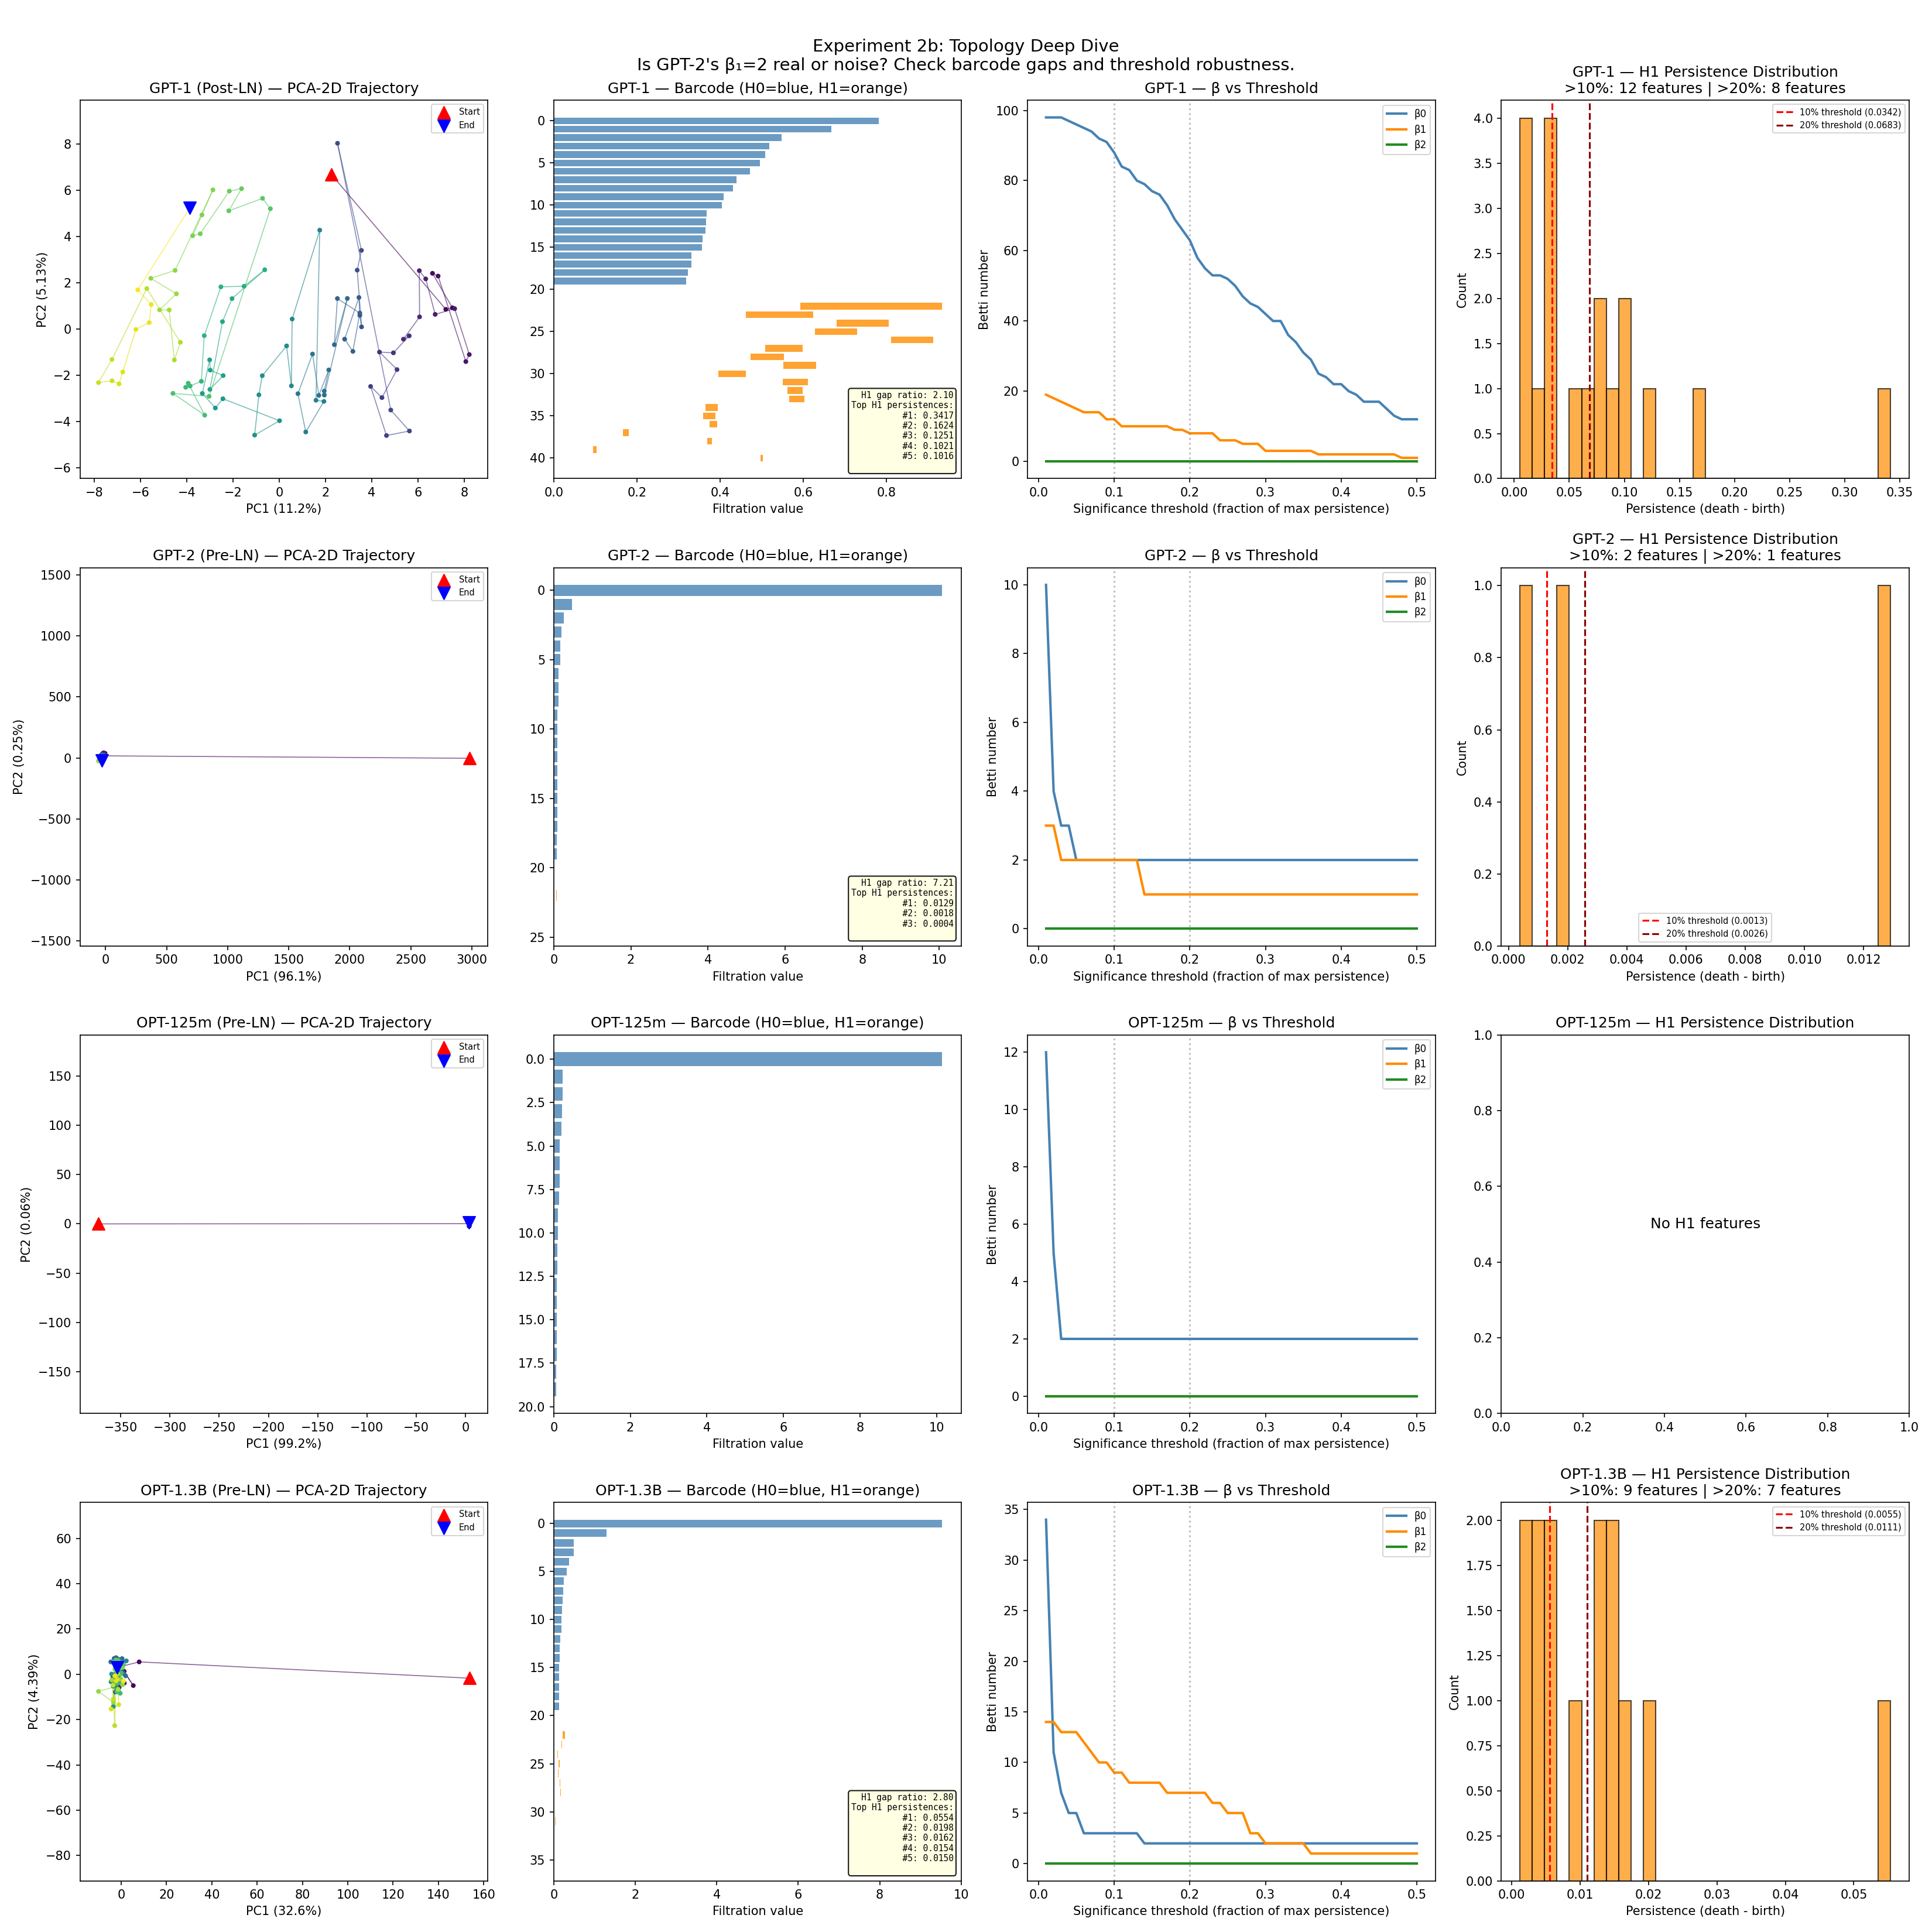
\includegraphics[width=\textwidth]{figures/fig1_barcode_deep_dive.png}
\caption{Topology deep dive across four models (rows: GPT-1, GPT-2, OPT-125m, OPT-1.3B). Columns: (a)~PCA-2D trajectory colored by token position; (b)~persistence barcode ($H_0$ blue, $H_1$ orange)---note the near-absence of orange bars for Pre-LN models; (c)~$\beta$ vs.\ significance threshold---$\beta_1$ drops to zero at moderate thresholds; (d)~$H_1$ persistence distribution---all bars concentrated near zero. GPT-1 (Post-LN, top row) shows a scattered, disconnected point cloud.}
\label{fig:barcode}
\end{figure}

Barcode analysis (Table~\ref{tab:h1bars}) shows that GPT-2's $H_1$ features have minuscule absolute persistence relative to $H_0$.

\begin{table}[h]
\centering
\caption{$H_1$ barcode statistics (GPT-2, PCA-2D, short text).}
\label{tab:h1bars}
\begin{tabular}{lccccr}
\toprule
Text & $H_1$ feat. & Gap ratio & Max $H_1$ pers. & Max $H_0$ pers. & Ratio \\
\midrule
Narrative   & 3 & 7.21  & 0.013 & 10.07 & 1\,:\,780 \\
Technical   & 2 & 1.51  & 0.003 &  9.22 & 1\,:\,3179 \\
Repetitive  & 2 & 41.46 & 0.005 &  8.53 & 1\,:\,1777 \\
\bottomrule
\end{tabular}
\end{table}

Despite the high gap ratio of 7.21 for narrative text, the $H_1$ features occupy a scale $780\times$ smaller than $H_0$. These are not topological holes in the manifold; they are fluctuations in a nearly 1-dimensional point cloud.

\subsubsection{High-Dimensional Analysis Confirms Noise}

With longer texts (${\sim}500$ tokens) and PCA dimensions from 2 to 20, $\beta_1$ increases monotonically with dimension (Table~\ref{tab:betadim}), the signature of high-dimensional sparsity artifacts rather than genuine topological structure.

\begin{table}[h]
\centering
\caption{$\beta_1$ by PCA dimension ($\alpha = 0.1$, narrative\_long).}
\label{tab:betadim}
\begin{tabular}{llccccc}
\toprule
Model & LN & PCA-2 & PCA-5 & PCA-10 & PCA-20 & Residual \\
\midrule
GPT-1    & Post & 16 & 64  & 130 & 173 & 176 \\
GPT-2    & Pre  & 34 & 70  & 156 & 194 & 167 \\
OPT-125m & Pre  & 0  & 95  & 161 & 209 & 156 \\
OPT-1.3B & Pre  & 46 & 59  & 104 & 131 & 129 \\
\bottomrule
\end{tabular}
\end{table}

If genuine topological features existed, $\beta_1$ would stabilize at the true number of independent loops as PCA dimension increases beyond the manifold's intrinsic dimension. No such stabilization is observed.

\begin{figure}[H]
\centering
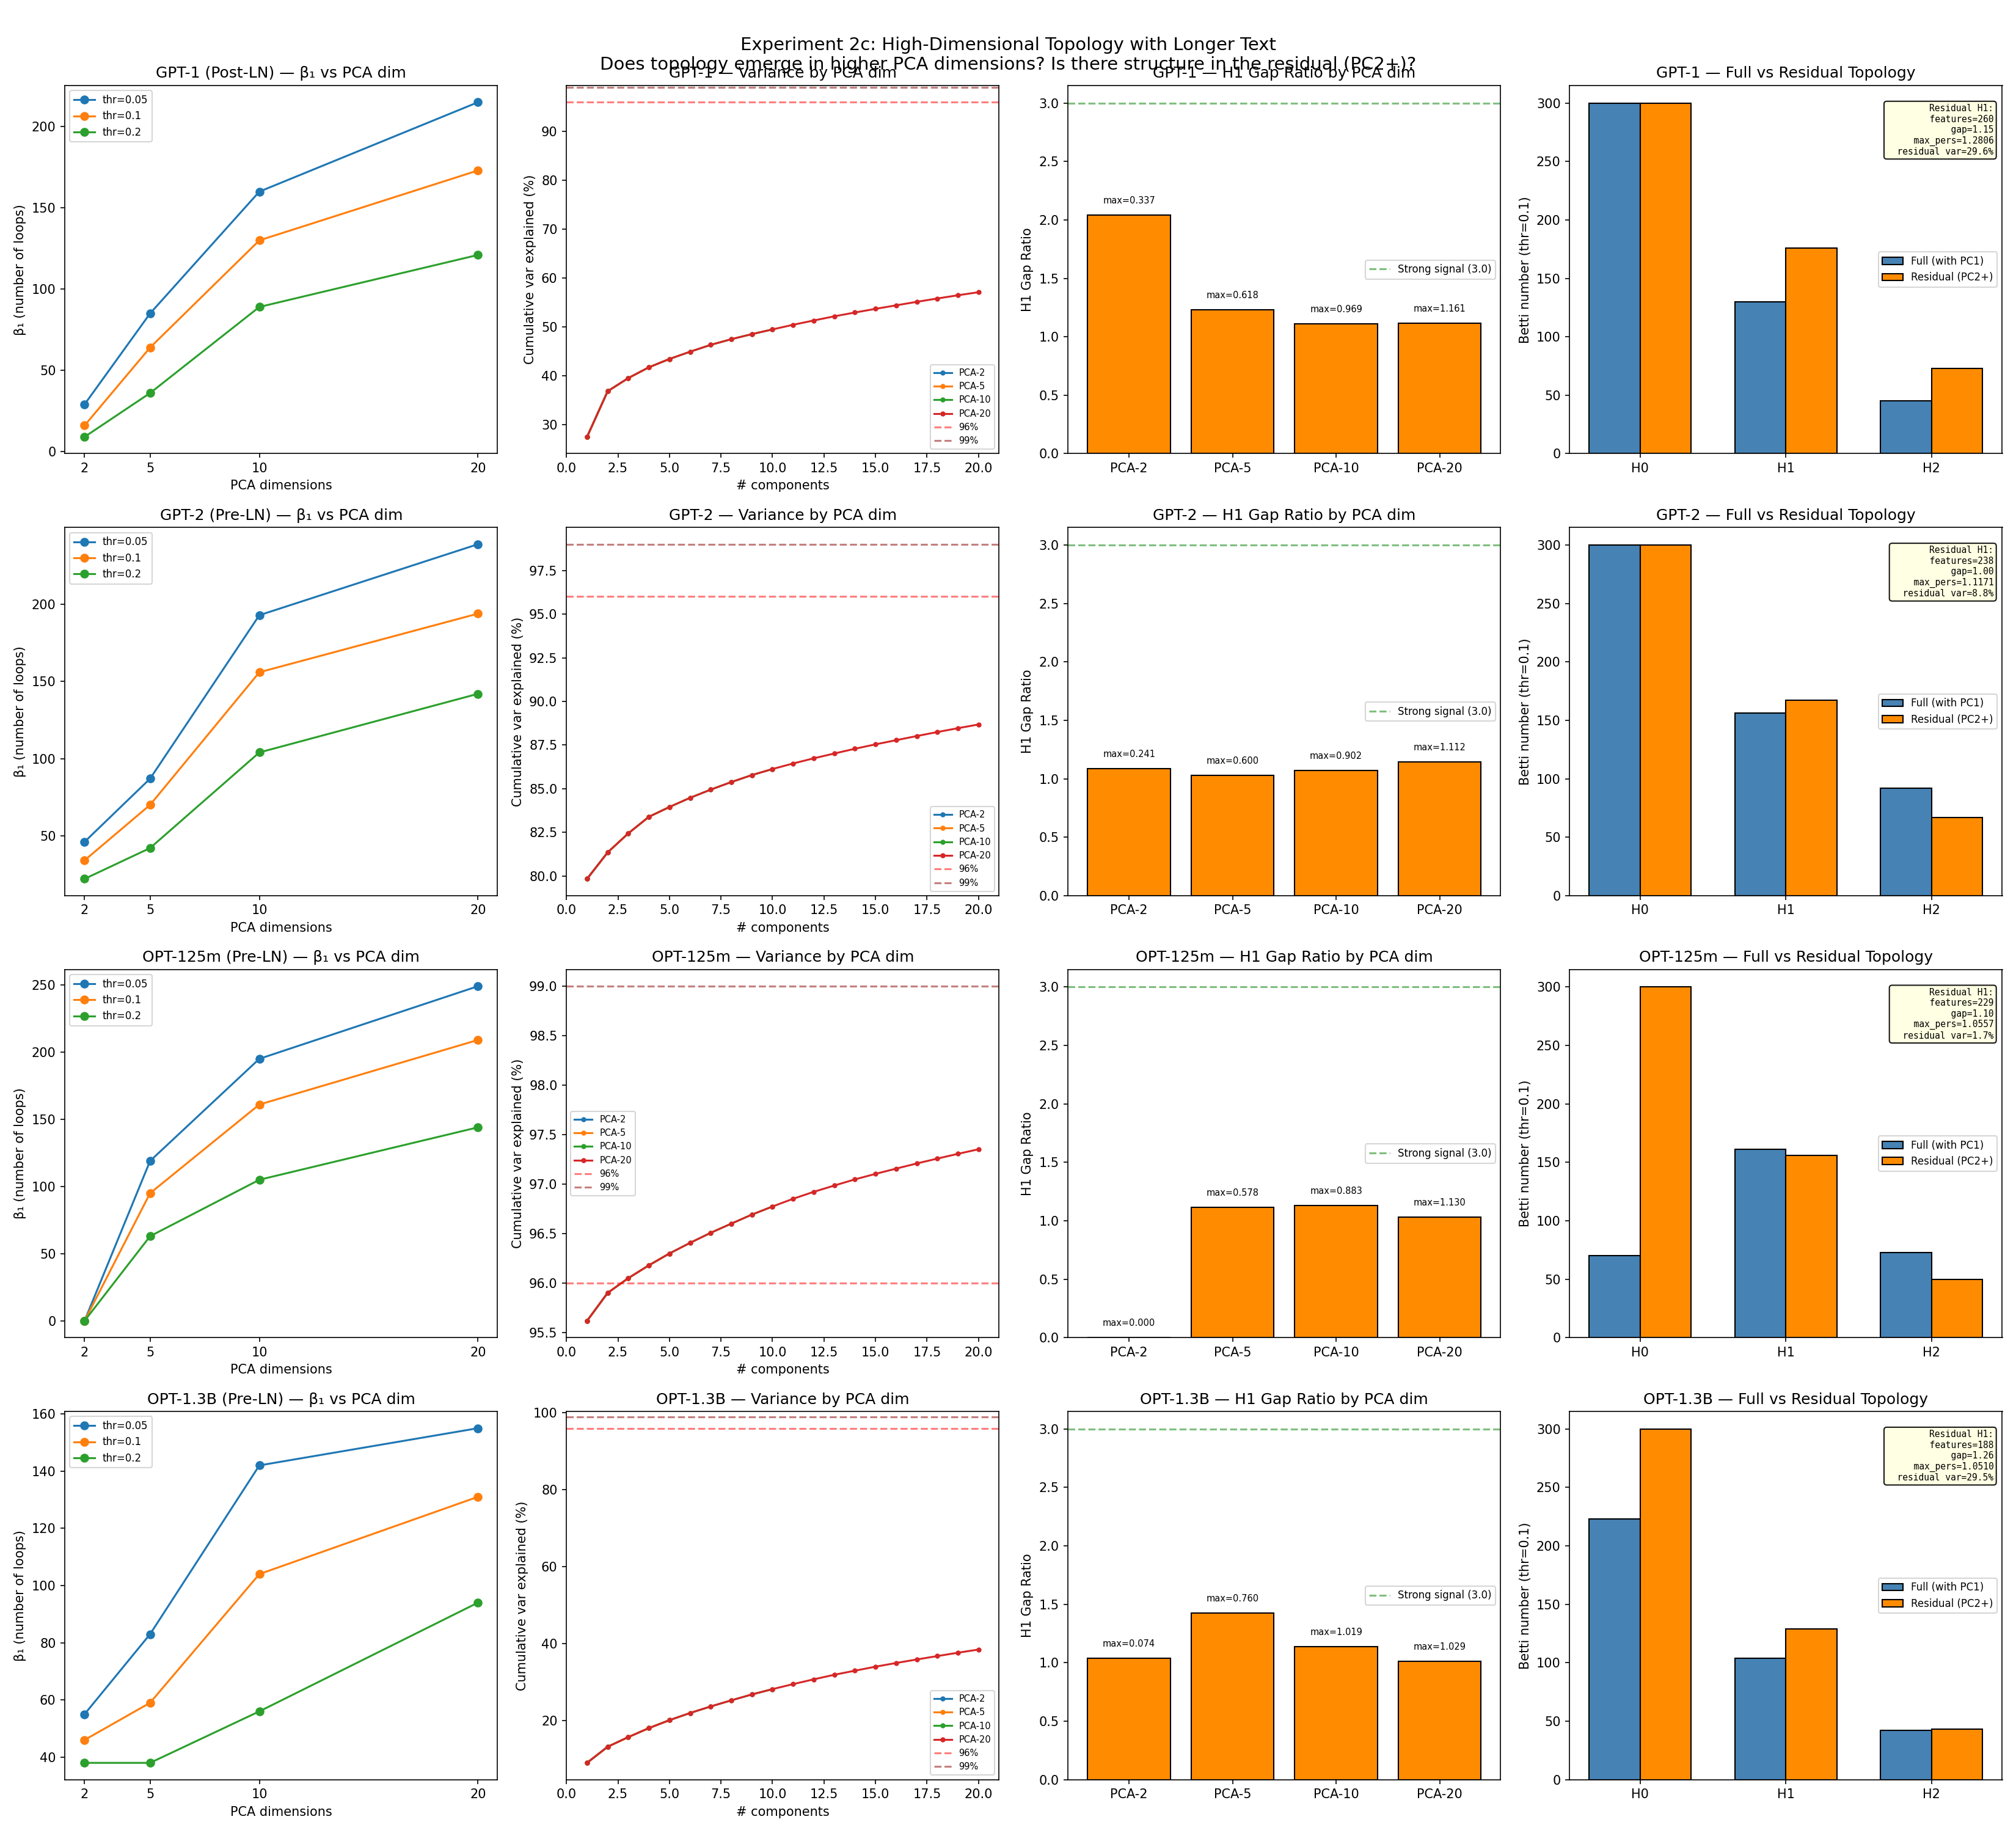
\includegraphics[width=\textwidth]{figures/fig2_multidim_topology.png}
\caption{High-dimensional topology analysis with longer text (${\sim}500$ tokens). Each row shows one model. Columns: (a)~$\beta_1$ vs.\ PCA dimension---monotonically increasing across all models, confirming sparsity-induced noise; (b)~cumulative PCA variance; (c)~$H_1$ gap ratio---no condition exceeds $G = 3$; (d)~full vs.\ residual (PC2+) Betti numbers.}
\label{fig:multidim}
\end{figure}

$H_1$ gap ratios are uniformly below 2.0 at PCA-5 and above (Table~\ref{tab:gapratio}), confirming that no $H_1$ feature stands out from the noise floor.

\begin{table}[h]
\centering
\caption{$H_1$ gap ratio by PCA dimension (narrative\_long).}
\label{tab:gapratio}
\begin{tabular}{lccccc}
\toprule
Model & PCA-2 & PCA-5 & PCA-10 & PCA-20 & Residual \\
\midrule
GPT-1    & 2.04 & 1.23 & 1.11 & 1.12 & 1.15 \\
GPT-2    & 1.09 & 1.03 & 1.07 & 1.14 & 1.00 \\
OPT-125m & --   & 1.11 & 1.13 & 1.03 & 1.10 \\
OPT-1.3B & 1.04 & 1.42 & 1.14 & 1.01 & 1.26 \\
\bottomrule
\end{tabular}
\end{table}

\subsubsection{Point Cloud Visualization}

\begin{figure}[H]
\centering
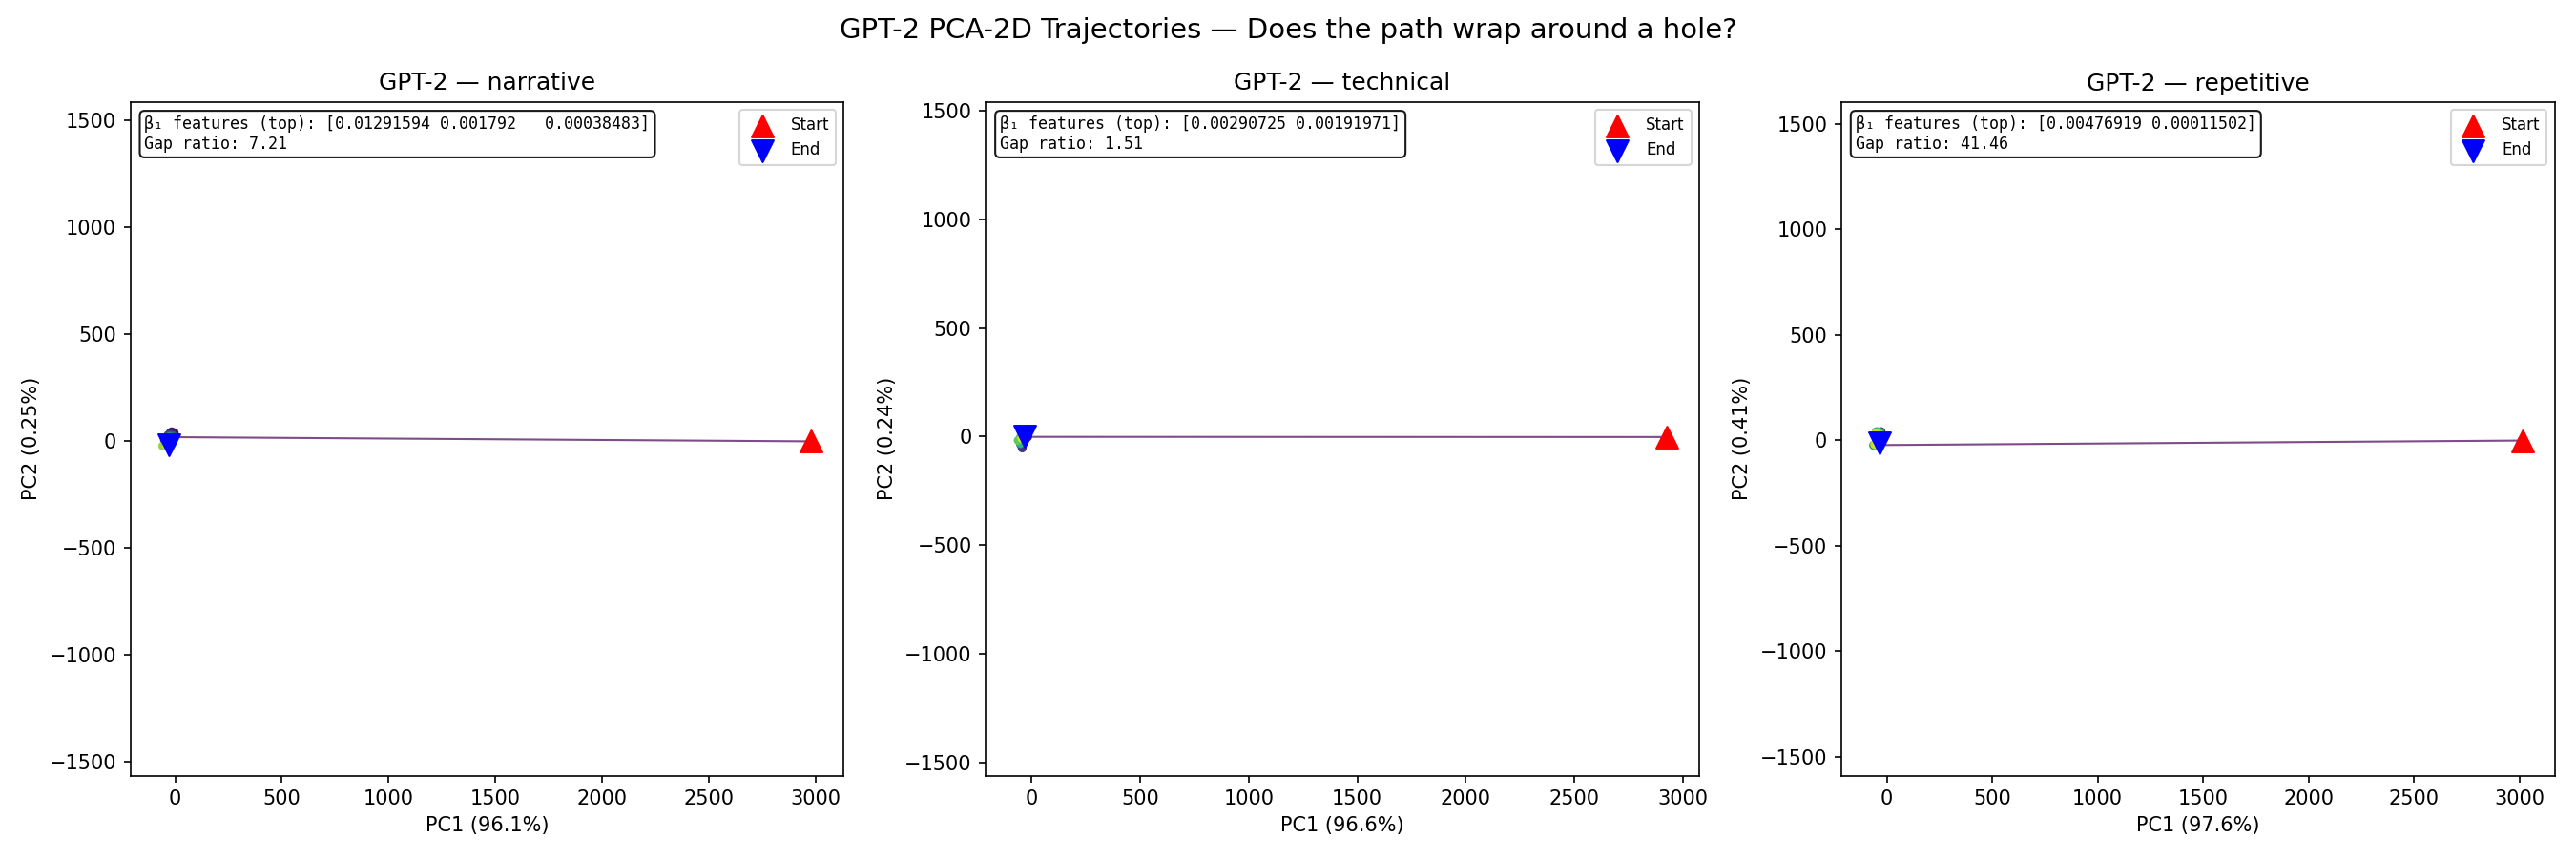
\includegraphics[width=\textwidth]{figures/fig3_gpt2_pointclouds.png}
\caption{GPT-2 hidden-state trajectories in PCA-2D for three text types. PC1 (horizontal) explains 96--98\% of variance; PC2 (vertical) contributes only 0.2--0.4\%. Trajectories are nearly 1-dimensional arcs from start (red~$\triangle$) to end (blue~$\triangledown$), with no visible wrapping or hole structure. The $\beta_1 = 2$ in Table~\ref{tab:betti} is an artifact of micro-fluctuations along this arc.}
\label{fig:pointcloud}
\end{figure}

Direct visualization of GPT-2 PCA-2D trajectories (Figure~\ref{fig:pointcloud}) confirms the quantitative findings: points distribute along a nearly horizontal line, with no visible hole or wrapping structure. The trajectory moves from start to end along the arc without completing a cycle.

\subsubsection{Post-LN Manifold is Disconnected}

GPT-1 (Post-LN) exhibits $\beta_0 = 89$--$300$ across conditions, indicating that its hidden states do not form a connected manifold. This is consistent with the finding that Post-LN distributes variance broadly (PCA-2D explains only 16--37\% of variance).

\subsection{The Arc's Principal Component is Hidden-State Norm}

Table~\ref{tab:probing} shows the five cross-text-replicated PC--feature associations from the probing analysis.

\begin{table}[h]
\centering
\caption{Cross-text replicated associations (GPT-2, Layer~6).}
\label{tab:probing}
\begin{tabular}{ccllcc}
\toprule
PC & Var.\ expl. & Feature & Narr.\ $r$ & Tech.\ $r$ & Replicated \\
\midrule
PC1 & 89.9--91.2\% & Hidden-state norm $\|h\|$ & $+0.999$ & $+0.999$ & Yes \\
PC2 & 0.55--0.69\% & Token absolute position  & $+0.900$ & $+0.905$ & Yes \\
PC3 & 0.48--0.55\% & Token character length    & $-0.592$ & $-0.619$ & Yes \\
PC3 & (same)       & Surprisal                & $-0.364$ & $-0.542$ & Yes \\
PC3 & (same)       & POS category (ANOVA $F$) & 67.2     & 63.1     & Yes \\
\bottomrule
\end{tabular}
\end{table}

The near-perfect correlation between PC1 and $\|h\|$ ($r = 0.999$) is the most striking finding. The ``arc'' in PCA space is not a trajectory through semantic space; it is the \textbf{direction of norm variation}. Pre-LN's residual accumulation structure causes hidden-state norms to vary systematically across token positions, and this norm variation dominates PCA.

\begin{figure}[H]
\centering
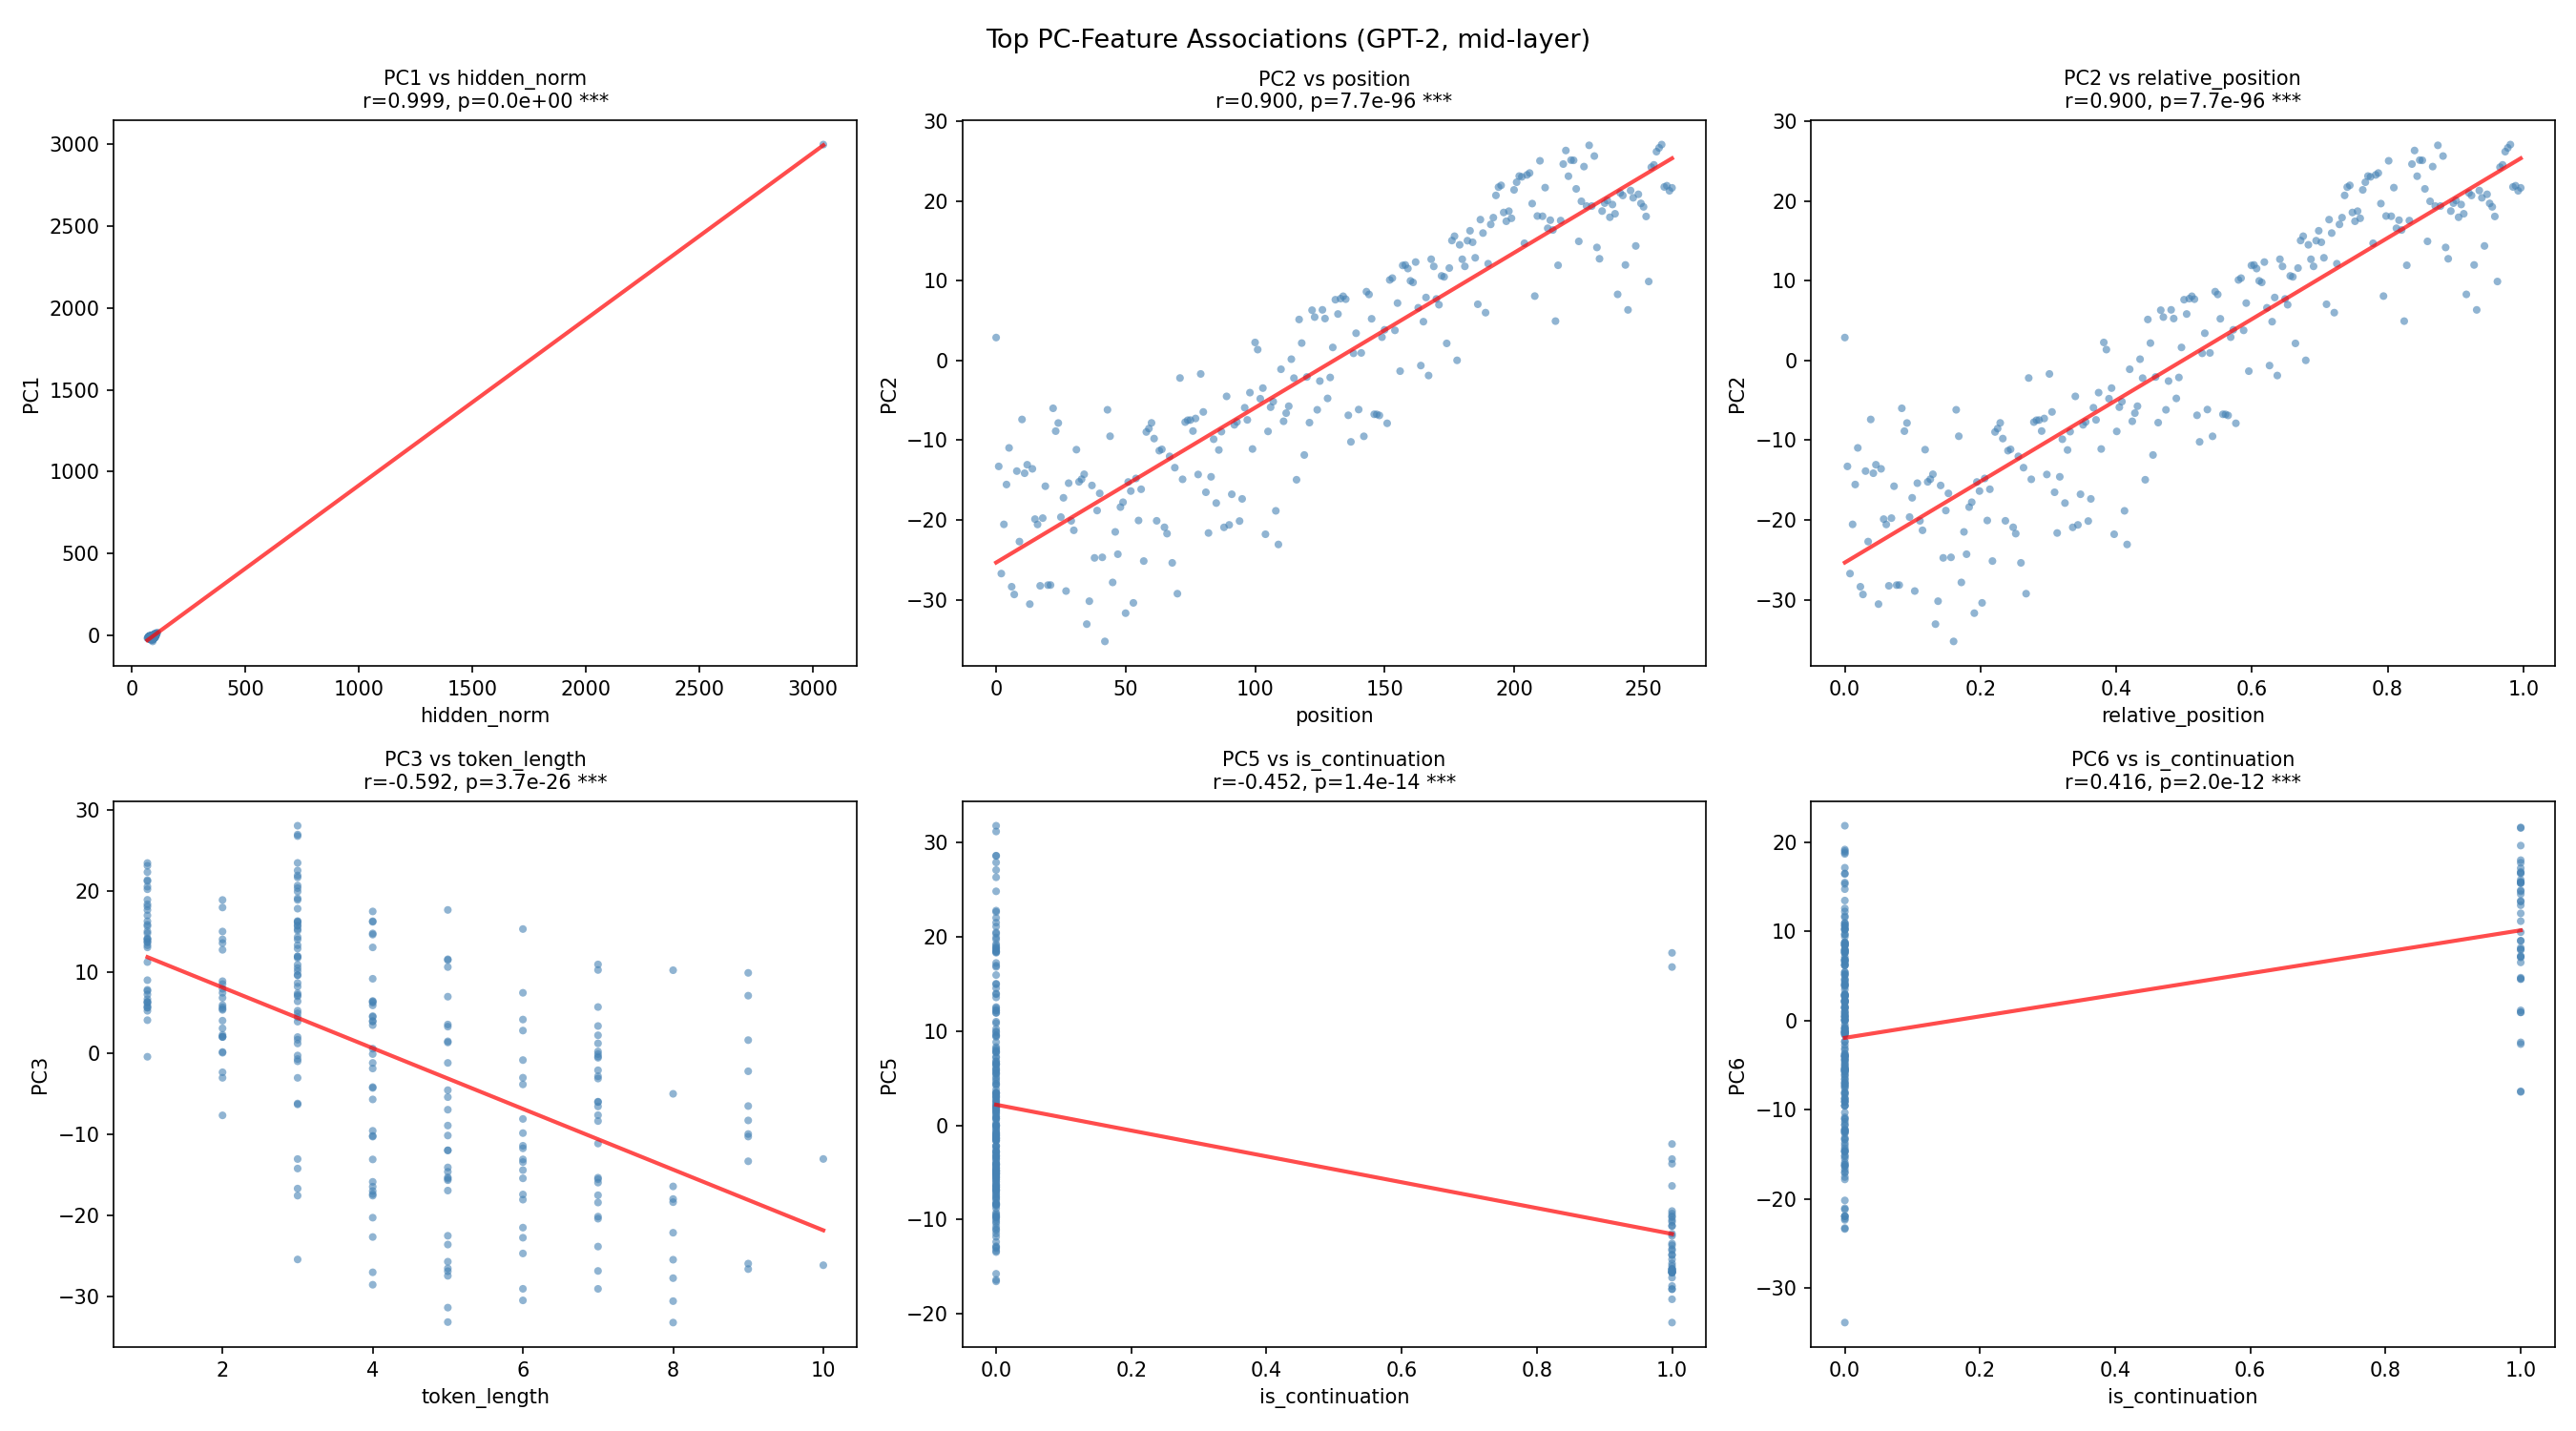
\includegraphics[width=\textwidth]{figures/fig4_pc_scatter.png}
\caption{Top six PC--feature associations (GPT-2, Layer~6, narrative text). Upper left: PC1 vs.\ hidden-state norm ($r = +0.999$)---near-perfect linearity confirming that the dominant PCA axis encodes norm. Upper middle/right: PC2 vs.\ token position ($r = +0.900$)---precise positional encoding in a sub-percent variance axis. Lower left: PC3 vs.\ token character length ($r = -0.592$). Lower middle/right: PC5 and PC6 vs.\ subword continuation flag.}
\label{fig:scatter}
\end{figure}

\subsection{Leading Residual Axis Encodes Token Position (GPT-2, Layer~6)}

In the canonical GPT-2 Layer~6 decomposition, PC2---the leading residual axis after norm---encodes absolute token position with $r = 0.90$ ($p \sim 10^{-96}$). Despite contributing only 0.55--0.69\% of total variance, this axis demonstrates that positional information from the embedding layer is preserved through six Transformer blocks and concentrated into a narrow spectral band of the hidden-state covariance matrix.

\subsection{Secondary Residual Axis Encodes Prediction Difficulty (GPT-2, Layer~6)}

In GPT-2 at Layer~6, the next residual axis (PC3) exhibits a dual encoding: token character length ($r = -0.59$) and surprisal ($r = -0.36$ to $-0.54$). The ANOVA $F$-statistic for POS category is 63--67 ($p \sim 10^{-38}$), with clear separation between punctuation (positive PC3), function words (intermediate), and content words (negative PC3). This ordering mirrors the information-theoretic hierarchy: punctuation is most predictable, content words least.

\begin{figure}[H]
\centering
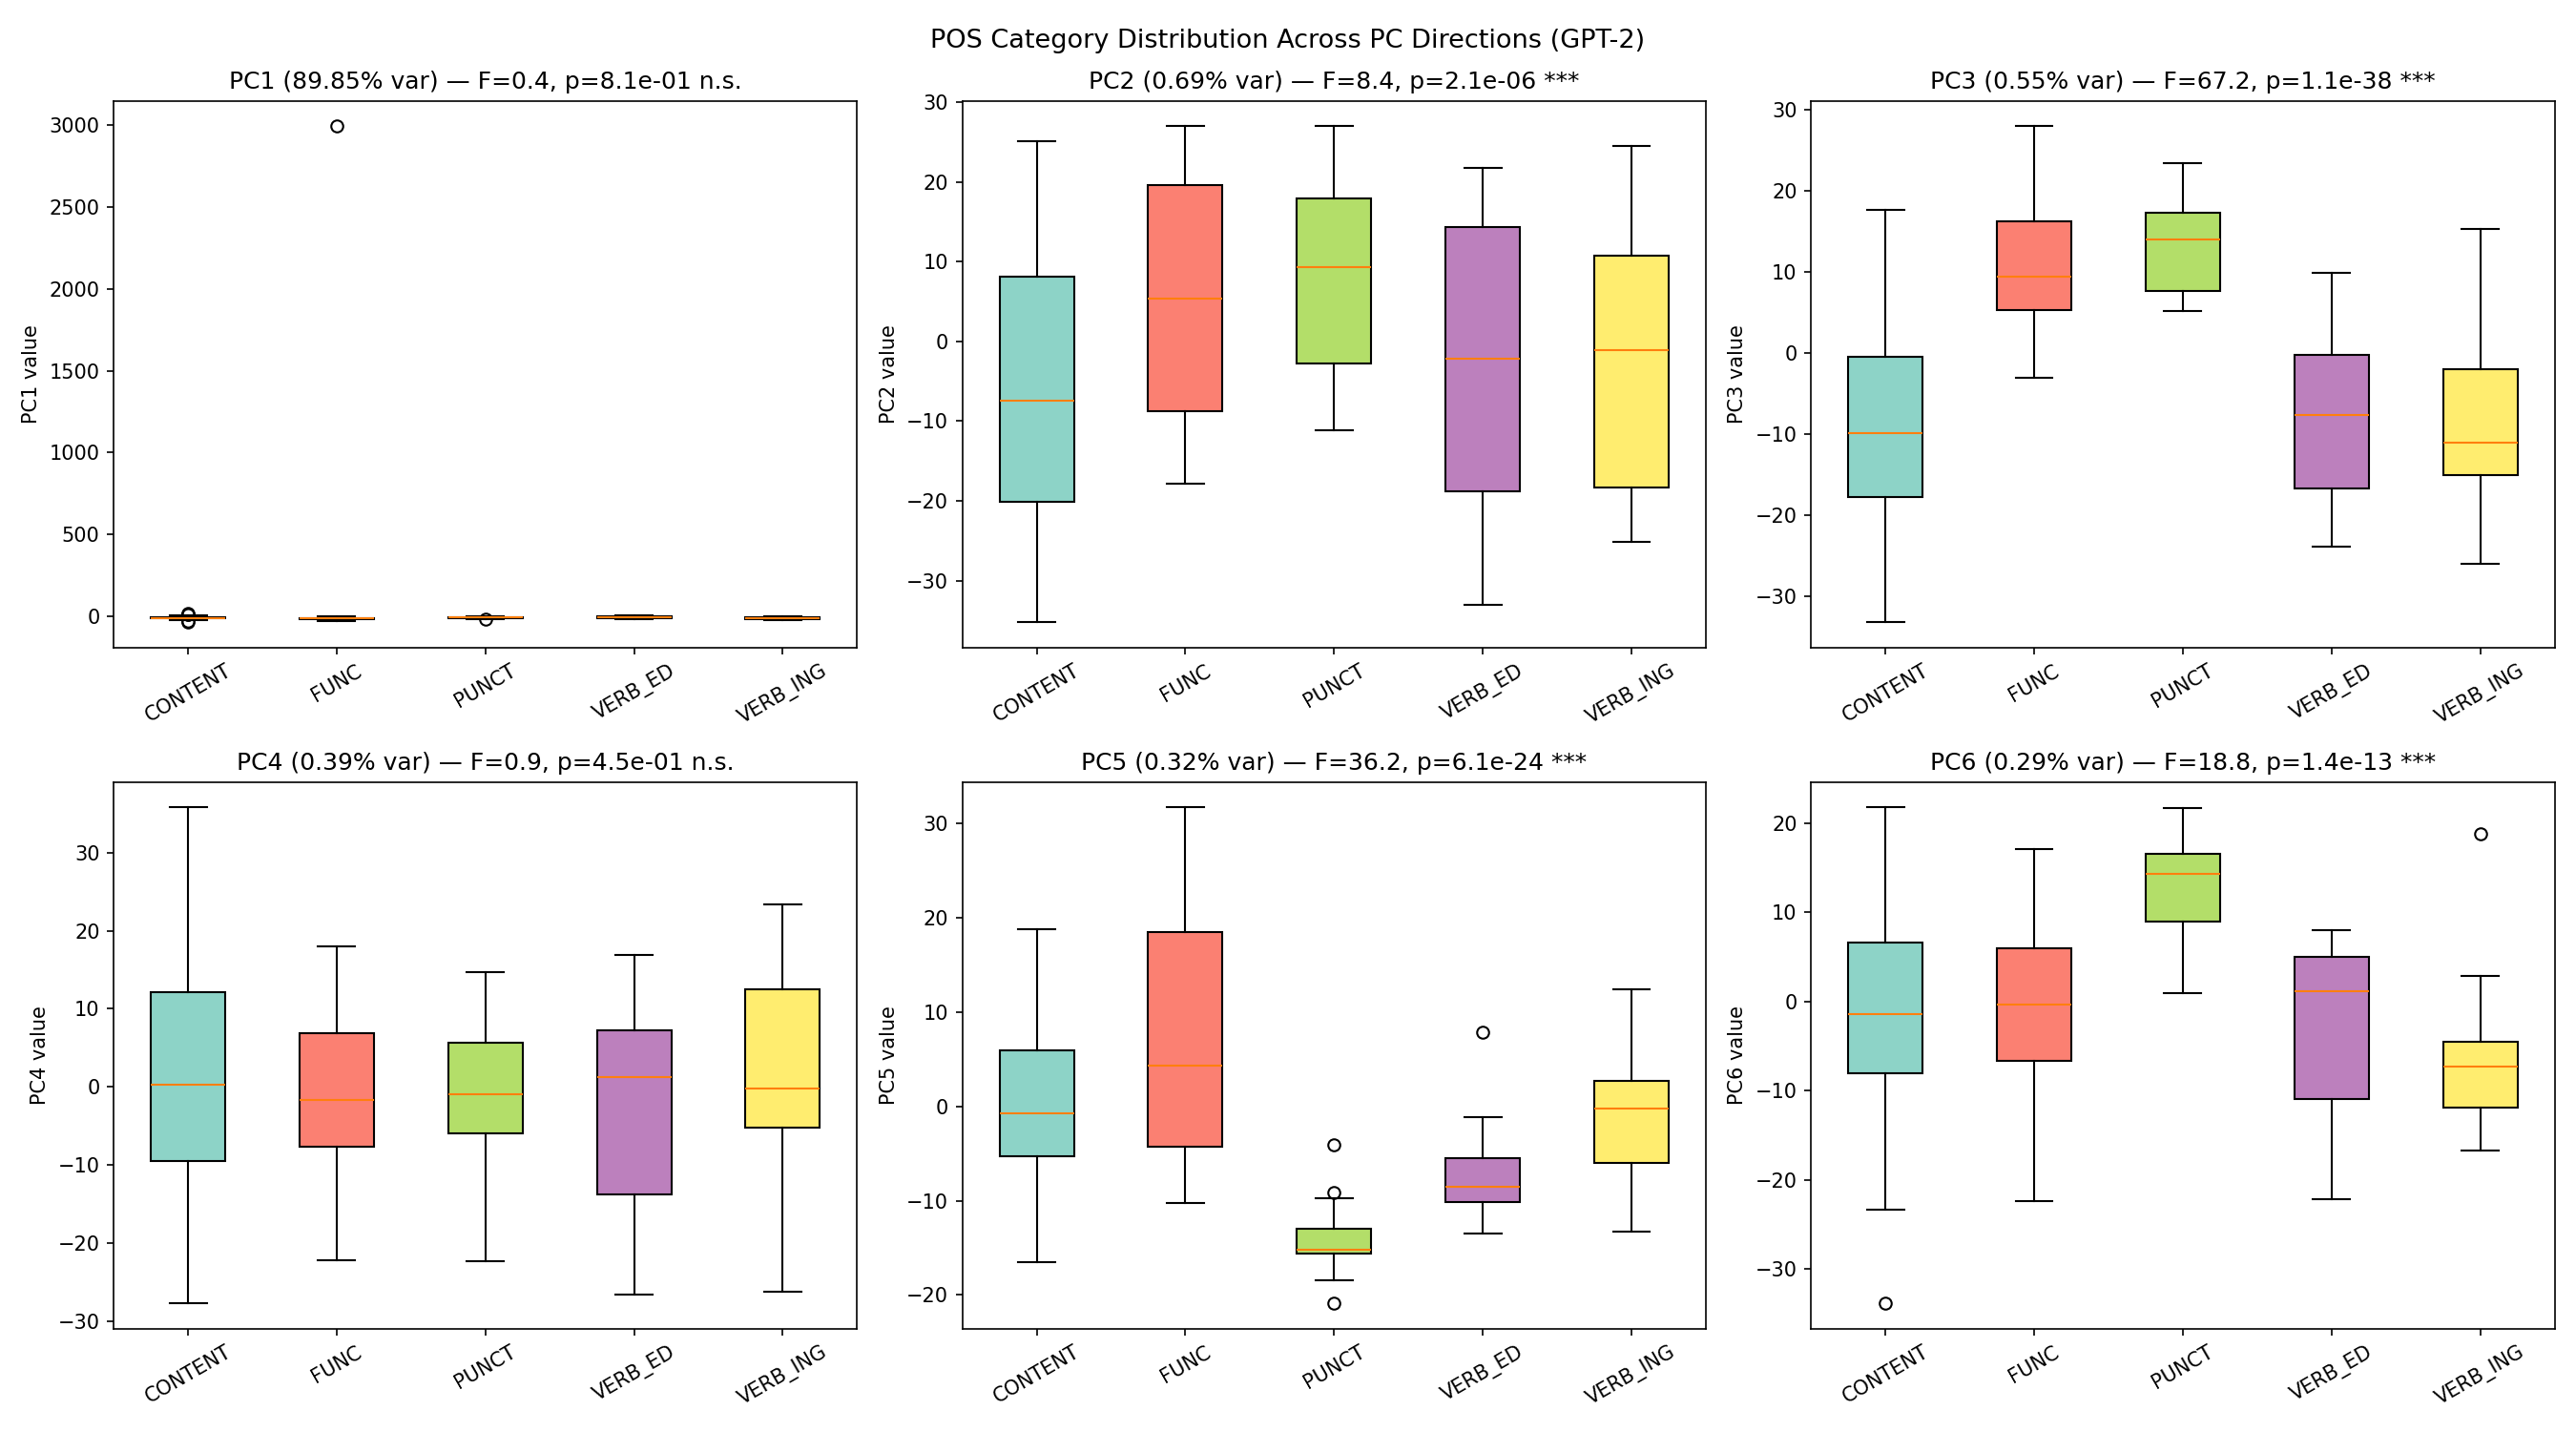
\includegraphics[width=\textwidth]{figures/fig5_pos_breakdown.png}
\caption{Distribution of PCA component values by part-of-speech category (GPT-2, Layer~6). PC1 shows no POS discrimination ($F = 0.4$, n.s.)---norm variation is POS-independent. PC3 shows the strongest POS discrimination ($F = 67.2$, $p \sim 10^{-38}$): punctuation tokens (\textsc{punct}) cluster at positive values, verb forms at negative values, and function words in between. This ordering recapitulates the information-theoretic hierarchy from most to least predictable.}
\label{fig:pos}
\end{figure}

\subsection{Higher Components Encode Subword and Morphological Features}

PC5 ($F = 36$) correlates with subword continuation status ($r = -0.45$), and PC6--PC8 show significant but less consistent POS discrimination. PC4 and PC9 are the only non-significant components for POS.

\subsection{Norm Normalization Reveals the Underlying Structure}

To directly verify that PC1 captures norm variation rather than linguistic content, we repeat the PCA analysis after normalizing each hidden state to unit norm: $\tilde{h}_t = h_t / \|h_t\|$. Table~\ref{tab:normnorm} compares the raw and normalized analyses.

\begin{table}[H]
\centering
\caption{Effect of norm normalization on PCA structure (GPT-2, Layer~6).}
\label{tab:normnorm}
\begin{tabular}{lcccccc}
\toprule
 & \multicolumn{3}{c}{Raw} & \multicolumn{3}{c}{Norm-Normalized} \\
\cmidrule(lr){2-4} \cmidrule(lr){5-7}
 & Var. & Encodes & $r$ / $F$ & Var. & Encodes & $r$ / $F$ \\
\midrule
PC1 & 94.8\% & Norm & $r{=}0.999$ & 7.0\% & Position & $r{=}0.805$ \\
PC2 & 0.36\% & Position & $r{=}0.863$ & 5.97\% & POS/difficulty & $F{=}115$ \\
PC3 & 0.32\% & POS/difficulty & $F{=}87.5$ & 4.67\% & (mixed) & $F{=}29.5$ \\
\bottomrule
\end{tabular}
\end{table}

Norm normalization reduces PC1 variance from 94.8\% to 7.0\%---an $87.8$ percentage-point drop---and completely eliminates the norm correlation ($r = 0.999 \to -0.071$). In the normalized space, position rises to PC1 ($r = 0.805$) and POS/difficulty rises to PC2 ($F = 115$, higher than the raw PC3's $F = 87.5$). This confirms that the original PCA is dominated by a single geometric axis (norm variation), and that removing it reveals and \emph{improves} the discriminability of linguistically meaningful features that are spectrally masked in the raw covariance structure.

\subsection{Layer-Wise Analysis: Emergence and Dissolution of the Arc}

We extend the probing analysis to all 12 transformer layers plus the embedding layer (Figure~\ref{fig:layerwise}). Table~\ref{tab:layerwise} reports PC1 statistics and the strongest position/POS associations at each depth.

\begin{figure}[H]
\centering
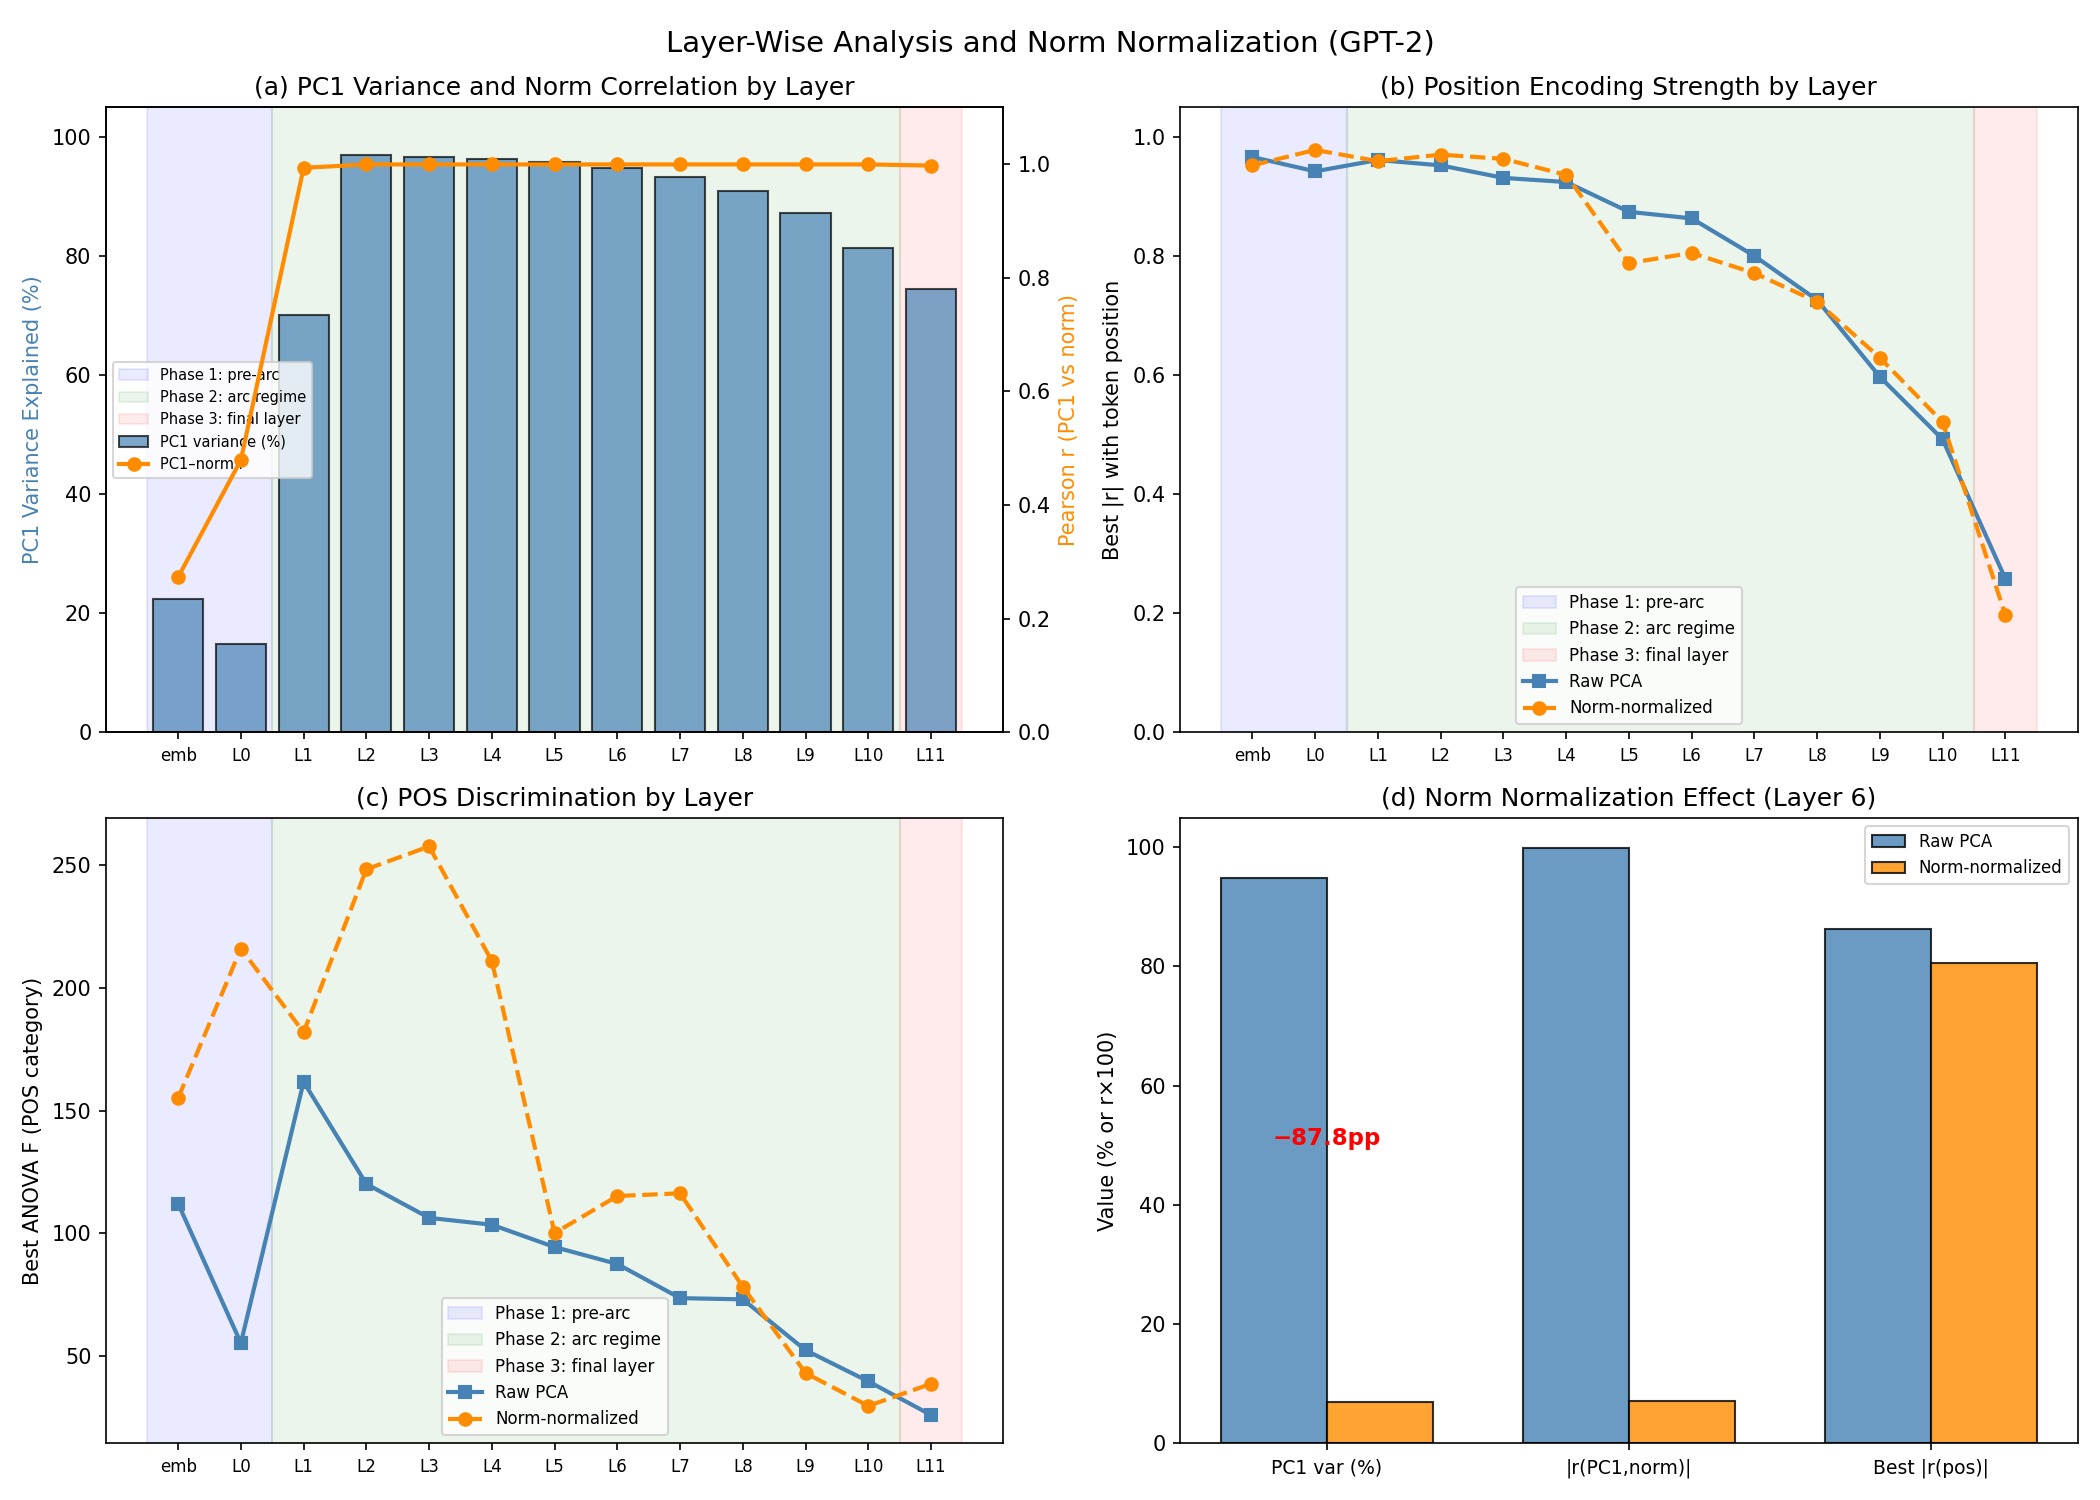
\includegraphics[width=\textwidth]{figures/fig7_layerwise.png}
\caption{Layer-wise PCA structure and norm normalization effect (GPT-2). Background shading marks three phases: pre-arc (blue, embed/L0), arc regime (green, L1--L10), and final layer (red, L11). (a)~PC1 variance (bars) and PC1--norm correlation (line)---L1 is the transition point where norm locks onto PC1. (b)~Position encoding strength decays through the arc regime; norm normalization (dashed orange) preserves position as the leading axis across all layers. (c)~POS discrimination peaks at L1 in raw PCA; norm normalization substantially improves POS $F$-values at all depths. (d)~Norm normalization at Layer~6 collapses PC1 variance by 87.8 percentage points.}
\label{fig:layerwise}
\end{figure}

\begin{table}[H]
\centering
\caption{Layer-wise PCA structure (GPT-2). For each layer: PC1 variance and norm correlation; strongest position correlation and its PC index; strongest POS $F$-statistic and its PC index.}
\label{tab:layerwise}
\begin{tabular}{lcccccc}
\toprule
Layer & PC1 var. & PC1--norm $r$ & Best $|r_\text{pos}|$ & PC & Best POS $F$ & PC \\
\midrule
embed & 22.4\% & $+0.273$ & 0.966 & \textbf{PC1} & 112.1 & PC5 \\
L0    & 14.8\% & $+0.479$ & 0.942 & \textbf{PC1} & 55.3  & PC2 \\
L1    & 70.0\% & $+0.993$ & 0.961 & PC2           & \textbf{161.7} & PC3 \\
L2    & 96.9\% & $+0.999$ & 0.952 & PC2           & 120.1 & PC3 \\
L3    & 96.6\% & $+0.999$ & 0.931 & PC2           & 106.3 & PC3 \\
L4    & 96.3\% & $+0.999$ & 0.924 & PC2           & 103.5 & PC3 \\
L5    & 95.7\% & $+0.999$ & 0.874 & PC2           & 94.4  & PC3 \\
L6    & 94.8\% & $+0.999$ & 0.863 & PC2           & 87.5  & PC3 \\
L7    & 93.3\% & $+0.999$ & 0.800 & PC2           & 73.6  & PC3 \\
L8    & 90.9\% & $+0.999$ & 0.726 & PC2           & 73.1  & PC3 \\
L9    & 87.2\% & $+0.999$ & 0.597 & PC2           & 52.4  & PC3 \\
L10   & 81.4\% & $+0.999$ & 0.492 & PC2           & 39.7  & PC3 \\
L11   & 74.5\% & $+0.997$ & 0.258 & PC5           & 26.0  & PC4 \\
\bottomrule
\end{tabular}
\end{table}

Three distinct phases are visible:

\paragraph{Phase~1: Embedding and L0 (pre-arc).} Position is directly encoded in PC1 ($r > 0.94$), and norm correlation is weak ($r < 0.48$). The arc structure has not yet formed; the dominant variation axis is positional.

\paragraph{Phase~2: L1--L10 (arc regime).} Starting at L1, PC1 abruptly locks onto norm ($r = 0.993$), absorbing 70--97\% of variance. Position is displaced to PC2, and POS/difficulty settles into PC3. POS discrimination peaks at L1 ($F = 161.7$) and decays monotonically through deeper layers. Position encoding also decays, from $r = 0.96$ (L1) to $r = 0.49$ (L10). This decay is consistent with deeper layers progressively integrating context, making individual token positions less salient.

\paragraph{Phase~3: L11 (final layer).} The arc partially dissolves: PC1 variance drops to 74.5\%, position encoding collapses ($r = 0.26$), and POS discrimination weakens to $F = 26$. The final layer exhibits a qualitatively different geometry, plausibly reflecting its closer coupling to the next-token prediction objective.

When norm normalization is applied (Table~\ref{tab:layerwisenorm}), position becomes the dominant PC1 feature at every layer ($r = 0.52$--$0.97$), supporting a consistent depth-wise hierarchy in which norm dominates raw PCA, while positional and POS structure become more prominent once norm variation is removed.

\begin{table}[H]
\centering
\caption{Norm-normalized layer-wise analysis (GPT-2). With norm removed, position consistently dominates PC1 and POS discrimination improves.}
\label{tab:layerwisenorm}
\begin{tabular}{lcccc}
\toprule
Layer & PC1 var. & Best $|r_\text{pos}|$ (PC) & Best POS $F$ (PC) \\
\midrule
embed & 23.8\% & 0.952 (PC1) & 155.1 (PC4) \\
L0    & 15.3\% & 0.978 (PC1) & 216.0 (PC2) \\
L1    & 13.7\% & 0.959 (PC1) & 181.9 (PC2) \\
L2    & 11.1\% & 0.970 (PC1) & 248.3 (PC2) \\
L3    &  9.1\% & 0.963 (PC1) & 257.6 (PC2) \\
L4    &  8.2\% & 0.936 (PC1) & 210.9 (PC2) \\
L5    &  7.3\% & 0.788 (PC1) & 100.1 (PC2) \\
L6    &  7.0\% & 0.805 (PC1) & 115.2 (PC2) \\
L7    &  7.3\% & 0.771 (PC1) & 116.3 (PC2) \\
L8    &  7.6\% & 0.723 (PC1) &  78.2 (PC2) \\
L9    &  8.8\% & 0.629 (PC1) &  43.1 (PC2) \\
L10   &  9.1\% & 0.521 (PC2) &  29.7 (PC2) \\
L11   & 49.3\% & 0.197 (PC2) &  38.7 (PC4) \\
\bottomrule
\end{tabular}
\end{table}

% ====================================================================
\section{Discussion}

\subsection{Recharacterizing the Low-Dimensional Structure}

Prior work characterized Pre-LN hidden states as residing on a ``low-dimensional manifold'' based on PCA concentration \citep{ethayarajh2019contextual,aghajanyan2021intrinsic}. Our results provide a more precise characterization:

\begin{quote}
In the tested Pre-LN models, middle-layer hidden states appear to be dominated by a single radial axis aligned with hidden-state norm (${\sim}90$\% of variance in GPT-2). After removing this axis, a structured residual subspace (${\sim}8$\% of variance) appears to encode positional and lexical information in approximately orthogonal directions. In GPT-2, this structure emerges after the first transformer block, stabilizes through middle layers, and weakens in the final layer.
\end{quote}

This recharacterization is not merely terminological. The distinction between a 2D manifold and a 1D arc with structured thickness has implications for how we understand representation capacity. A 2D manifold suggests two degrees of freedom for encoding; a structured arc suggests a hierarchy: one dominant axis (norm/scale) with secondary axes carrying different types of linguistic information at much smaller variance scales.

Cross-model validation (Table~\ref{tab:crossmodel}) shows that PC1--norm alignment is consistent across all tested Pre-LN architectures, while the assignment of linguistic features to specific PC indices varies by model.

\begin{table}[H]
\centering
\caption{Cross-model comparison of PCA structure (mid-layer, narrative text). PC1--norm alignment ($|r| > 0.96$) is observed across all 11 tested Pre-LN models from 124M to 40B parameters, spanning 5 architecture families. Position and POS encoding appear in all cases but at model-dependent PC indices. OPT models are consistent outliers with weaker PC1 dominance.}
\label{tab:crossmodel}
\begin{tabular}{llccccl}
\toprule
Model & LN & PC1 var. & PC1--norm $r$ & Best $|r_\text{pos}|$ & Best POS $F$ & Notes \\
\midrule
GPT-2     & Pre-LN       & 94.8\% & $+0.999$ & 0.863 (PC2) & 87.5 (PC3) & Canonical \\
Pythia-410M & Pre-LN     & 96.5\% & $-1.000$ & 0.528 (PC3) & 18.1 (PC5) & PCs shuffled \\
Qwen2-0.5B & Pre-LN (RMS)& 98.7\% & $+1.000$ & 0.562 (PC3) & 21.3 (PC3) & RMSNorm same \\
OPT-1.3B  & Pre-LN       & 27.0\% & $+0.923$ & 0.640 (PC3) & 15.5 (PC2) & OPT-specific \\
Pythia-2.8B & Pre-LN     & 83.1\% & $+0.999$ & 0.665 (PC2) & 40.6 (PC3) & Pattern holds \\
\midrule
\multicolumn{7}{l}{\emph{7B-scale models (validated on Google Colab, T4 GPU):}} \\
Mistral-7B  & Pre-LN (RMS) & 90.0\% & $-0.999$ & 0.571 (PC2) & 19.1 (PC3) & 7B confirmed \\
Qwen2-7B    & Pre-LN (RMS) & 99.5\% & $-1.000$ & 0.552 (PC2) & 15.8 (PC3) & 7B confirmed \\
Pythia-6.9B & Pre-LN       & 80.3\% & $+1.000$ & 0.454 (PC2) & 43.4 (PC3) & 7B confirmed \\
\midrule
\multicolumn{7}{l}{\emph{13B+ models (validated on Google Colab, Blackwell GPU):}} \\
Pythia-12B  & Pre-LN       & 80.5\% & $+1.000$ & 0.449 (PC2) & 37.3 (PC3) & 12B confirmed \\
OPT-13B     & Pre-LN       & 71.0\% & $+0.962$ & 0.372 (PC4) & 22.2 (PC2) & OPT weaker again \\
Qwen2.5-14B & Pre-LN (RMS) & 99.7\% & $-1.000$ & 0.553 (PC2) & 16.7 (PC4) & Qwen highest \\
Falcon-40B  & Pre-LN       & 98.1\% & $-1.000$ & 0.555 (PC3) & 18.1 (PC5) & 40B confirmed \\
\bottomrule
\end{tabular}
\end{table}

PC1--norm alignment holds across all 11 tested Pre-LN models ($|r| > 0.96$), spanning 124M to 40B parameters and five distinct architecture families (GPT-2, GPT-NeoX/Pythia, Qwen, Mistral, Falcon). Falcon-40B---the largest model tested ($d = 8192$, 60 layers)---shows $|r| = 1.000$ with PC1 variance of 98.1\%, demonstrating that norm dominance persists at the 40B scale. The Qwen family shows the highest concentration across all scales tested (98.7\% at 0.5B, 99.5\% at 7B, 99.7\% at 14B), with concentration \emph{increasing} with model size. The OPT family is a consistent outlier with weaker dominance (27\% at 1.3B, 71\% at 13B), likely reflecting OPT-specific architectural choices.

\begin{figure}[H]
\centering
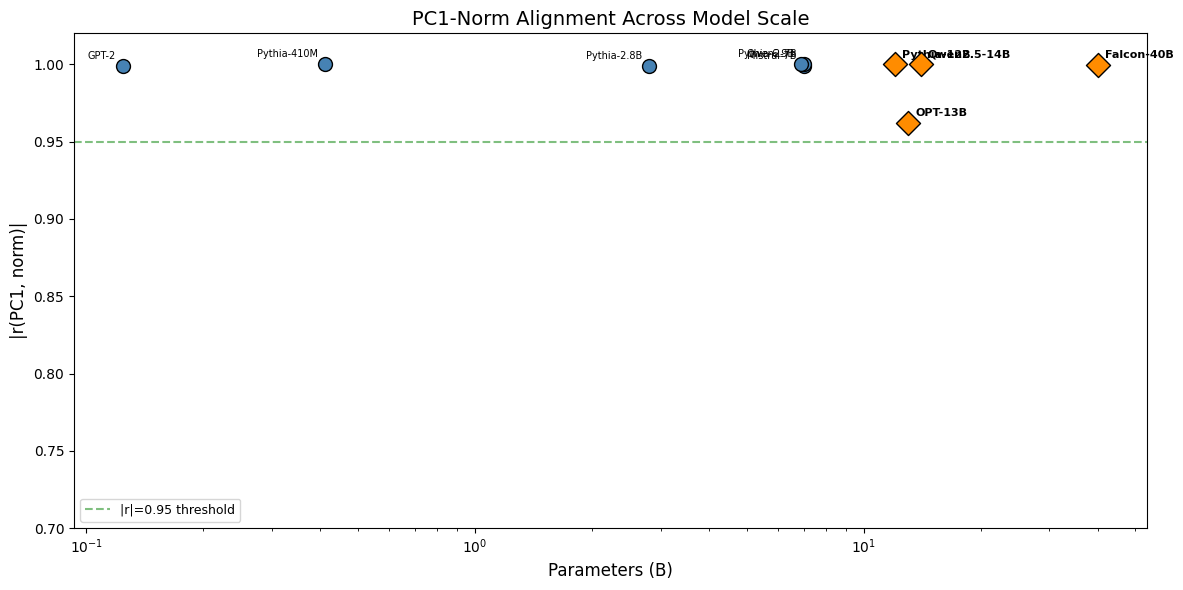
\includegraphics[width=0.85\textwidth]{figures/fig12_large_scale.png}
\caption{PC1--norm alignment ($|r|$) across model scale, from GPT-2 (124M) to Falcon-40B (40B). Blue circles: models tested locally ($\leq 2.8$B). Orange diamonds: models tested on Colab GPU (6.9B--40B). All 12 models exceed the $|r| = 0.95$ threshold (dashed green line). OPT-13B is the weakest but still above 0.96.}
\label{fig:large_scale}
\end{figure} The weaker PC1 dominance in OPT-1.3B ($d_\text{model} = 2048$, PC1 variance 27\%) suggests that higher-dimensional models distribute norm variation less anisotropically, consistent with the observation that intrinsic dimensionality grows with model scale \citep{aghajanyan2021intrinsic}.

\subsection{Why is PC1 the Norm?}

Pre-LN applies LayerNorm before each sublayer:
\begin{equation}
    h_{l+1} = h_l + F_l(\mathrm{LN}(h_l))
\end{equation}
The sublayer output $F_l(\mathrm{LN}(h_l))$ is added to $h_l$ without normalization of the sum. This induces substantial norm variation across layers and token positions, making it the dominant axis of hidden-state covariance. Post-LN normalizes after addition ($h_{l+1} = \mathrm{LN}(h_l + F_l(h_l))$), suppressing this effect and distributing variance more uniformly---consistent with our finding that Post-LN hidden states are not concentrated on a low-dimensional subspace.

This norm dominance has a methodological implication: PCA-based analyses of Pre-LN Transformer representations are primarily capturing norm variation, not semantic structure. The semantically relevant structure resides in the residual subspace beyond the dominant norm axis, which collectively accounts for less than 10\% of variance but carries linguistically interpretable information.

\subsection{Layer-Wise Profiles are Model-Specific}

Layer-wise analysis at 7B scale reveals that while the three-phase structure (pre-arc $\to$ arc regime $\to$ final-layer dissolution) is shared across all tested models, the \emph{shape} of the PC1 variance profile is highly model-specific. We identify three distinct patterns:

\begin{itemize}
    \item \textbf{Plateau type} (GPT-2): Rapid rise at L1, sustained high variance (95--97\%), gradual descent to 75\% at the final layer.
    \item \textbf{Funnel type} (Pythia-6.9B, Mistral-7B): Peak in early layers followed by monotonic decay to ${<}11$\% at the final layer.
    \item \textbf{Cliff type} (Qwen2-7B): Extended plateau at 99\%+ for 23 layers (L3--L25), then abrupt collapse to 19\% in the final two layers.
\end{itemize}

\begin{figure}[H]
\centering
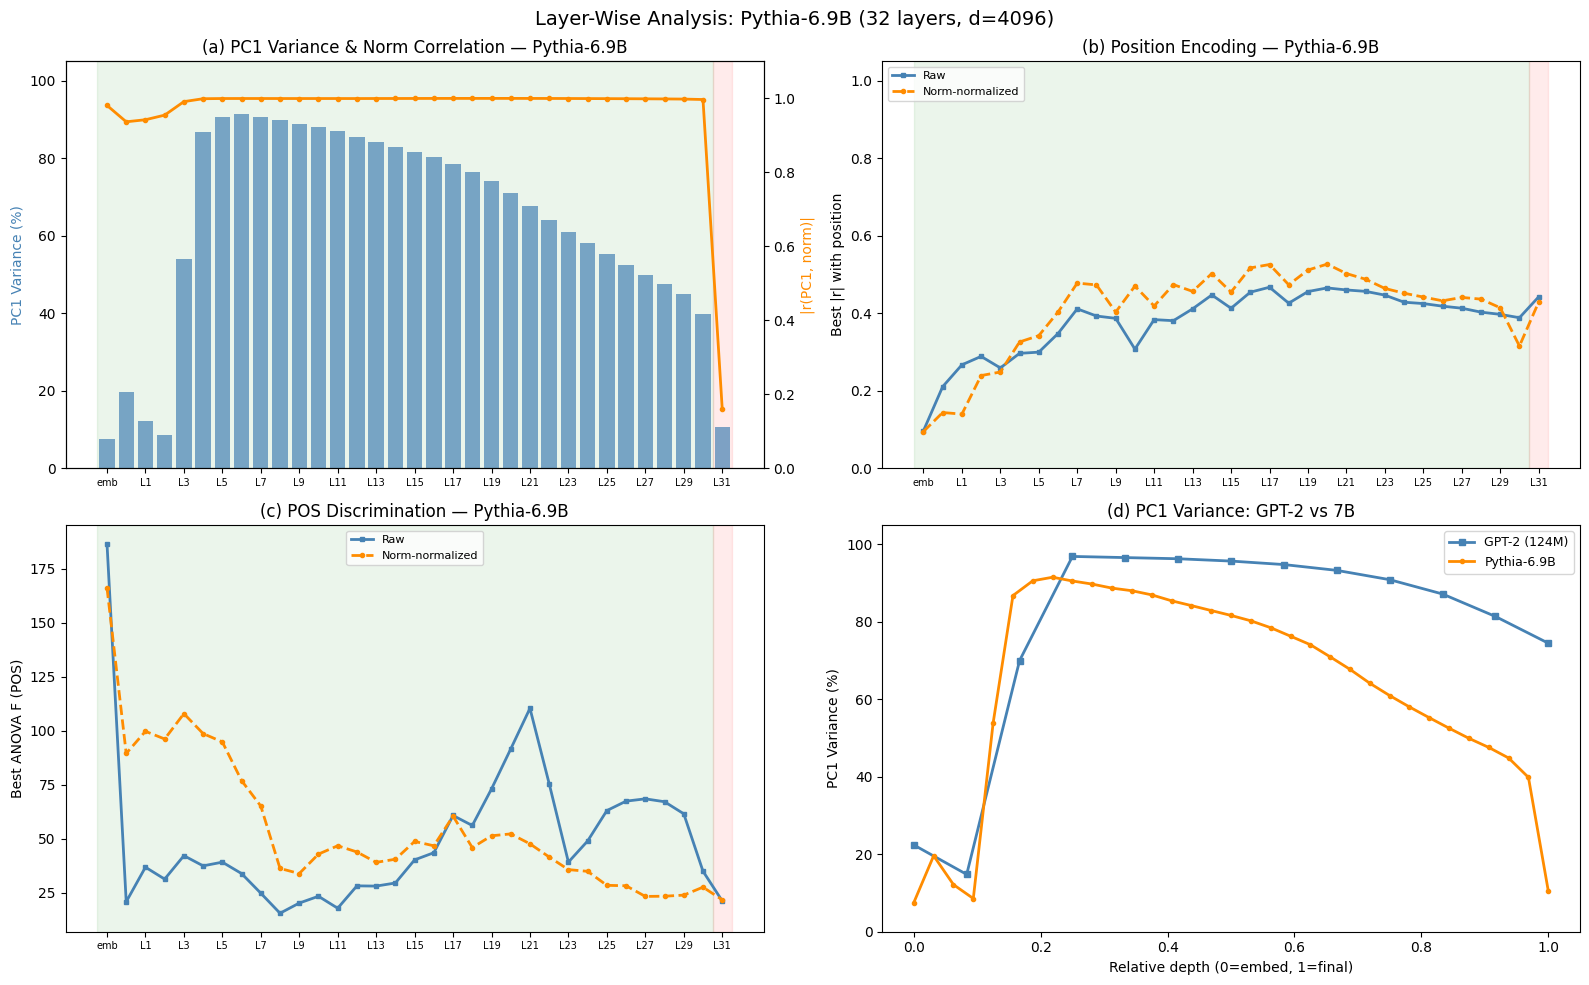
\includegraphics[width=\textwidth]{figures/fig9_layerwise_pythia.png}
\caption{Layer-wise PCA analysis of Pythia-6.9B (32 layers, $d{=}4096$). The funnel pattern is evident: PC1 variance peaks at L6 (91.5\%) and decays monotonically to 10.5\% at L31. The final layer shows near-complete dissolution ($|r_\text{norm}| = 0.16$). Compare with GPT-2's plateau pattern in (d).}
\label{fig:pythia_layerwise}
\end{figure}

\begin{figure}[H]
\centering
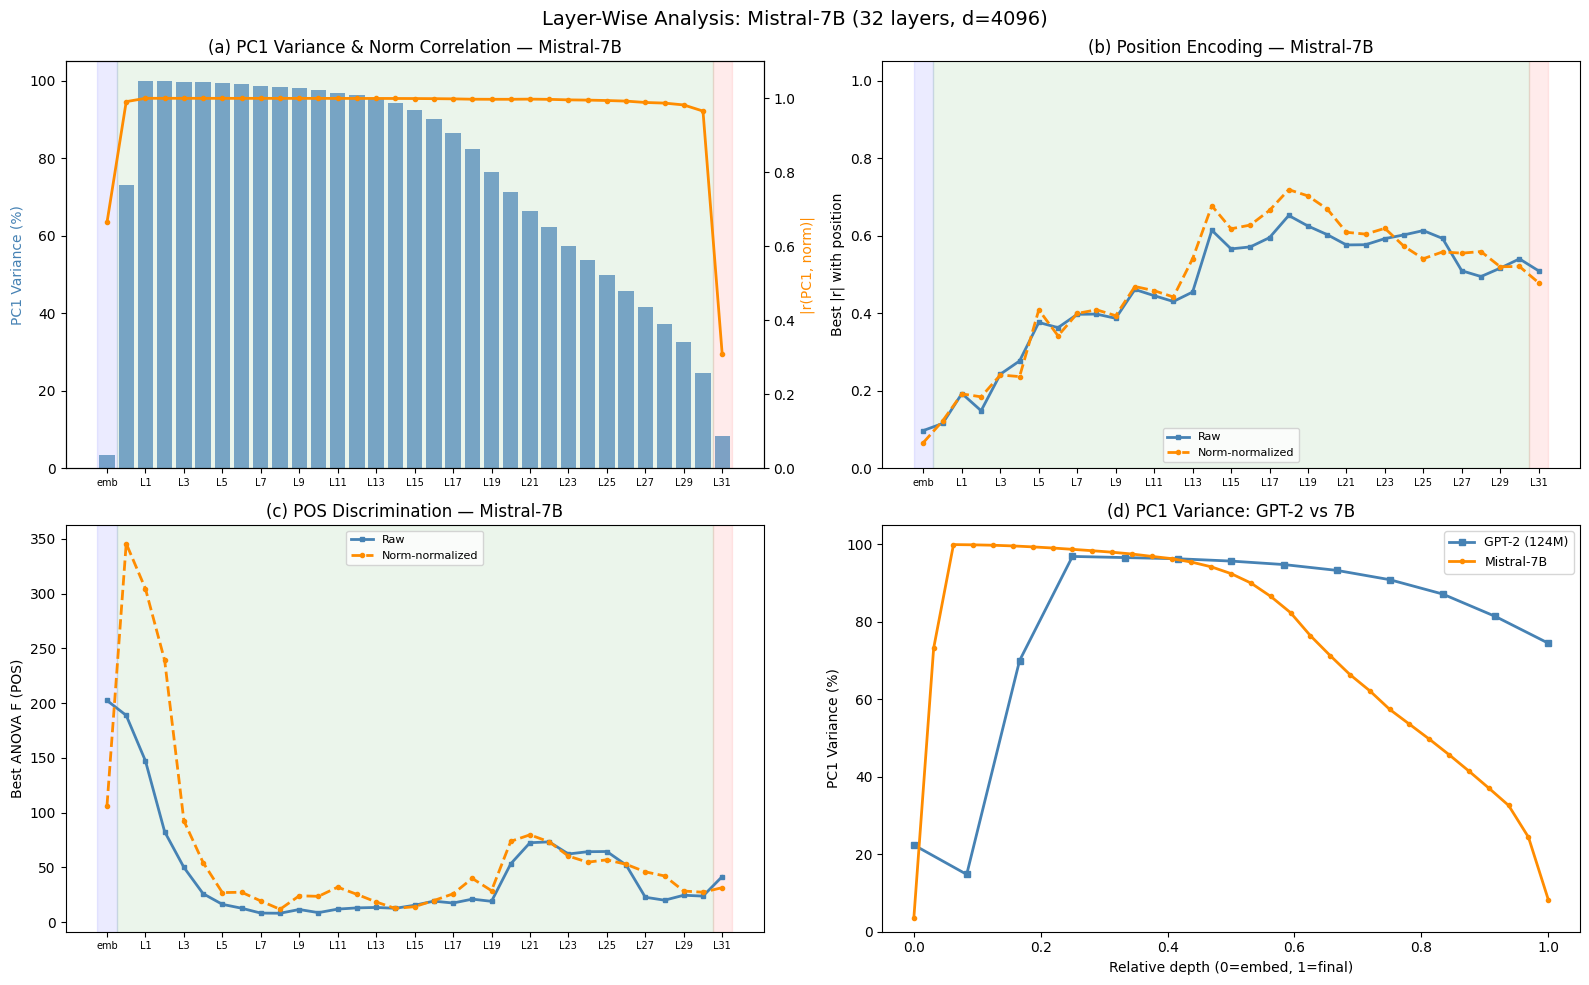
\includegraphics[width=\textwidth]{figures/fig10_layerwise_mistral.png}
\caption{Layer-wise PCA analysis of Mistral-7B (32 layers, $d{=}4096$, RMSNorm). PC1 hits 100.0\% at L1---the most extreme anisotropy of any tested model---then decays monotonically to 8.3\% at L31. Position encoding peaks in the middle layers (L18, $r{=}0.65$). The (d) panel directly overlays GPT-2 and Mistral-7B profiles, showing the qualitatively different shapes.}
\label{fig:mistral_layerwise}
\end{figure}

Notably, Mistral-7B reaches PC1${}=100.0$\% at L1---the most extreme anisotropy observed in any model. We initially hypothesized that this was driven by RMSNorm (which lacks bias terms), but Qwen2-7B (also RMSNorm) shows only 9.0\% at L1, \textbf{rejecting the RMSNorm hypothesis}. The extreme early concentration in Mistral may instead reflect its use of Sliding Window Attention, which constrains early-layer context integration, though this remains speculative.

\begin{figure}[H]
\centering
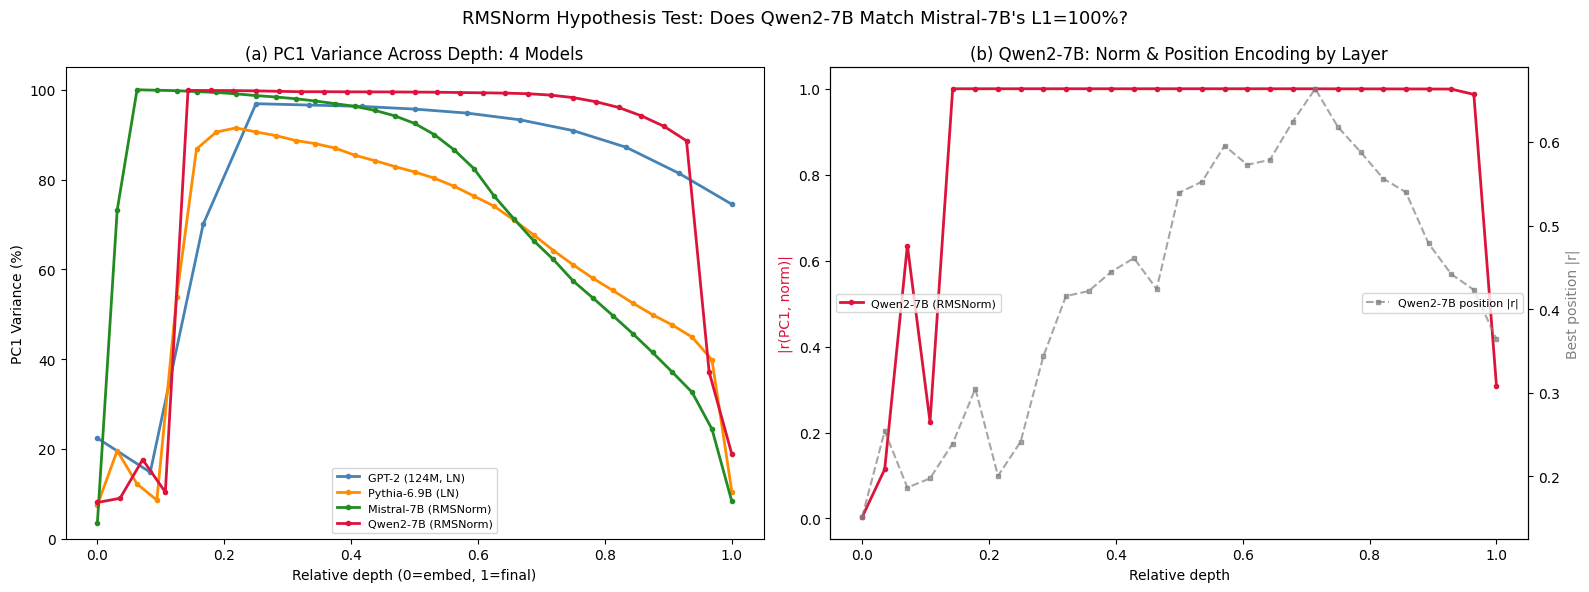
\includegraphics[width=\textwidth]{figures/fig11_qwen2_rmsnorm.png}
\caption{RMSNorm hypothesis test. (a)~PC1 variance across depth for all four models. Mistral-7B (green) and Qwen2-7B (red) both use RMSNorm but show strikingly different profiles: Mistral hits 100\% at L1 while Qwen2 reaches only 9\%. The Qwen2 ``cliff'' pattern (99\%+ for 23 layers, then abrupt collapse at L26) is distinct from both the Mistral funnel and the GPT-2 plateau. (b)~Qwen2-7B norm correlation and position encoding by layer.}
\label{fig:rmsnorm_test}
\end{figure}

The final-layer dissolution is dramatically more severe at 7B scale: PC1 variance drops to 8--19\% (vs.\ 75\% in GPT-2), and the PC1--norm correlation falls below $r = 0.31$. The 32-layer models appear to undergo a qualitative representational shift in their final layers that is absent in the 12-layer GPT-2, plausibly reflecting greater specialization for next-token prediction after deeper processing.

\subsection{A Natural Coordinate System for Hidden States}

\begin{figure}[H]
\centering
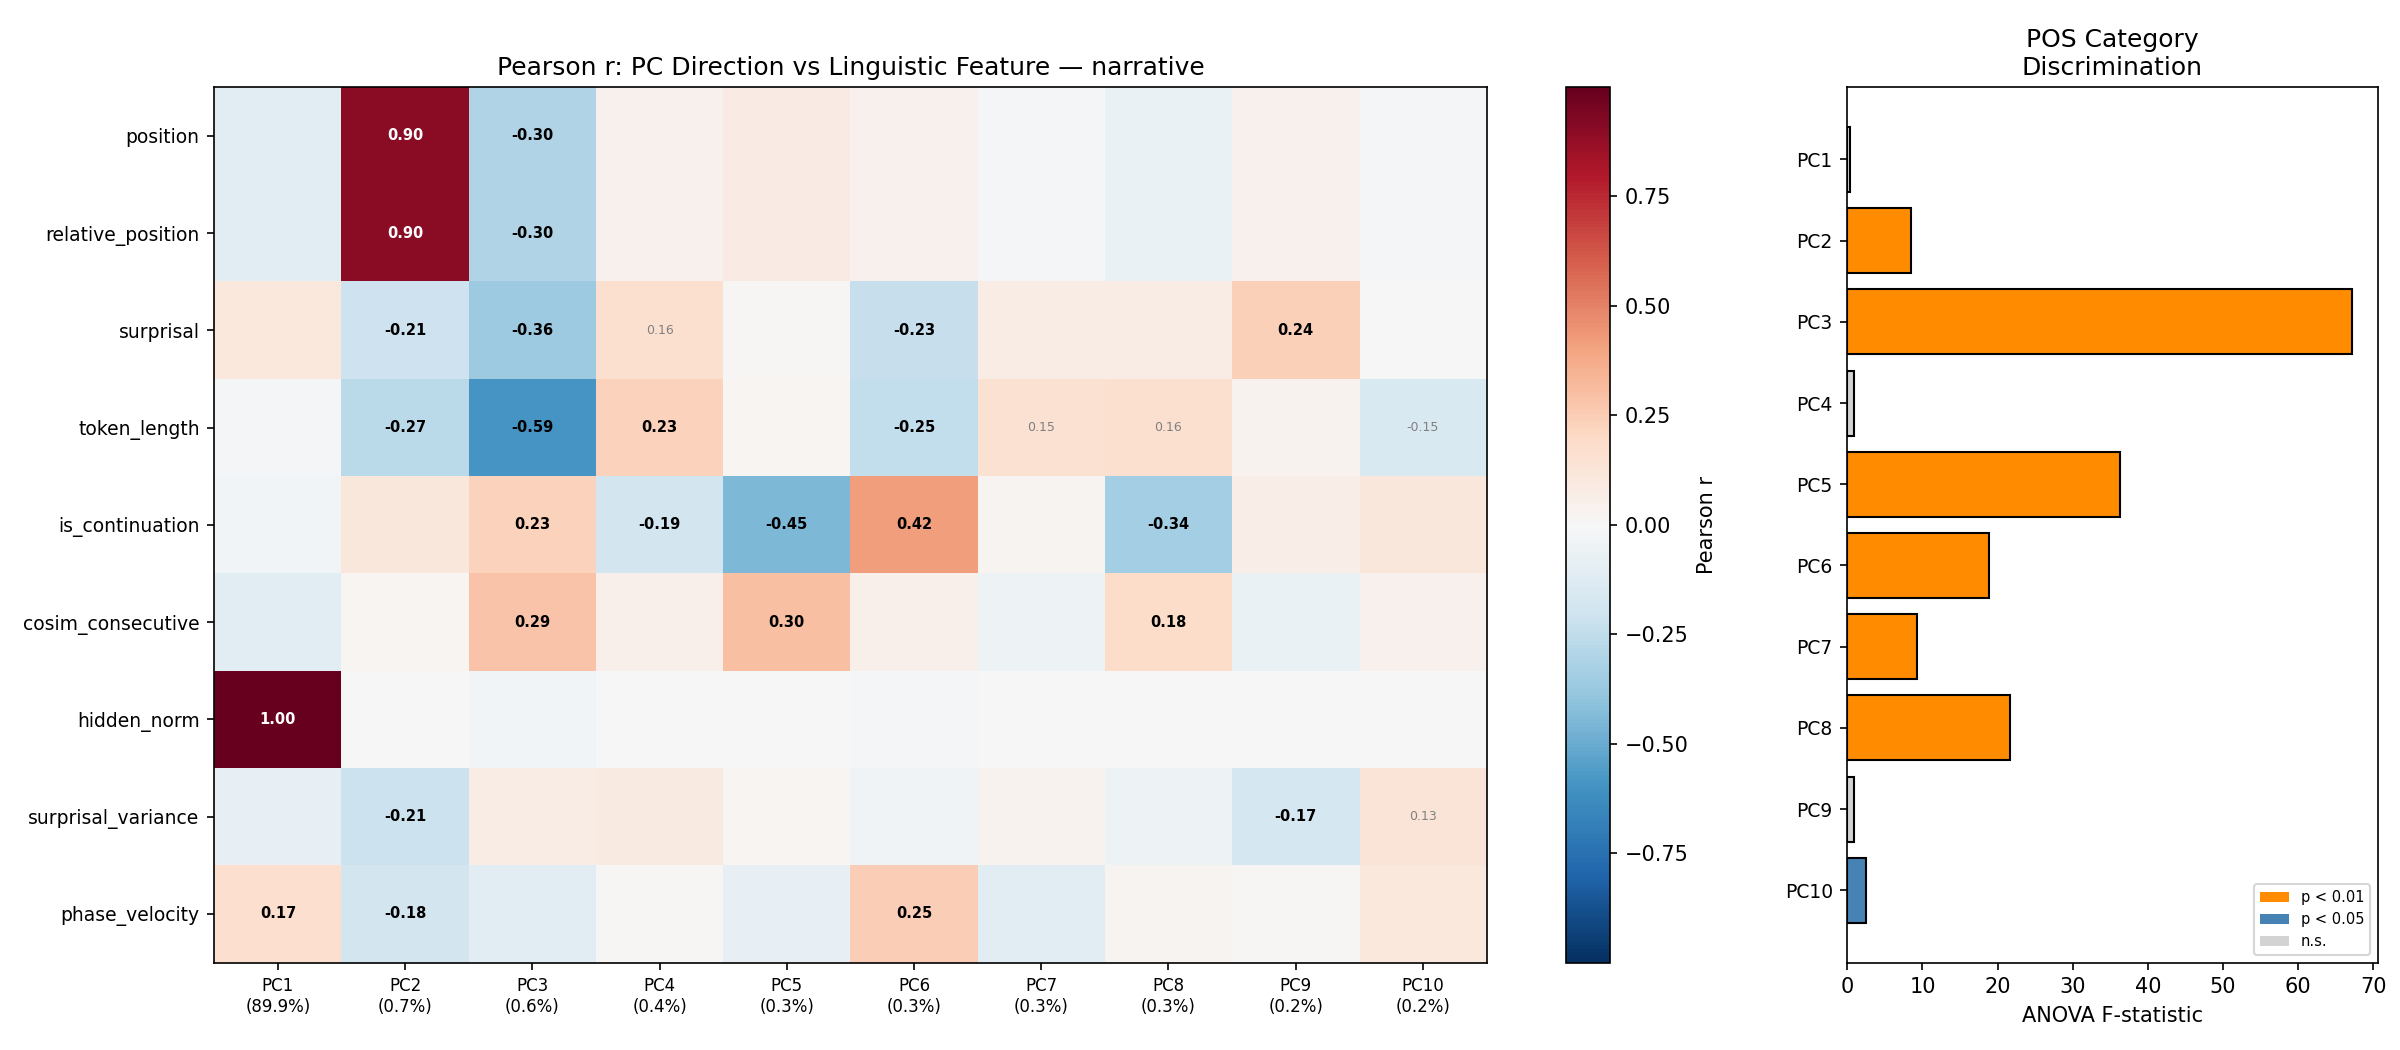
\includegraphics[width=\textwidth]{figures/fig6_heatmap.png}
\caption{Left: Pearson correlation heatmap between PCA components (columns) and linguistic features (rows) for GPT-2, narrative text. Significant correlations ($p < 0.01$) are annotated. The block-diagonal structure is striking: PC1 correlates exclusively with norm, PC2 with position, PC3 with surprisal/token length. Right: ANOVA $F$-statistic for POS category discrimination by PC direction. PC3 ($F = 67$) and PC5 ($F = 36$) are the strongest POS discriminators; PC1 and PC4 are non-significant.}
\label{fig:heatmap}
\end{figure}

The probing results (Figure~\ref{fig:heatmap}) suggest that PCA decomposition provides a linguistically interpretable coordinate system:

\begin{table}[h]
\centering
\caption{Functional hierarchy of Pre-LN hidden-state variation. The dominant axis consistently encodes norm; residual axes encode position and lexical features, but their PC indices are model- and layer-dependent.}
\label{tab:coords}
\begin{tabular}{lclp{5cm}}
\toprule
Axis type & Typical variance & Encodes & Stability \\
\midrule
Dominant radial & ${\sim}90$\% (raw) & Hidden-state norm $\|h\|$ & Consistent across tested Pre-LN models \\
Leading residual & ${\sim}0.5$--$5$\% & Token position & Present in all models; PC index varies \\
Secondary residual & ${\sim}0.5$--$4$\% & Lexical difficulty / POS & Present in all models; PC index varies \\
Higher residual & ${<}\,0.3$\% each & Subword, morphology & Weaker, less stable \\
\bottomrule
\end{tabular}
\end{table}

This decomposition is notable for several reasons. First, the axes are orthogonal by construction (PCA), meaning each encodes an independent dimension of variation. Second, the mapping is consistent across text types, suggesting it reflects architectural properties rather than input-specific patterns. Third, the ordering by variance is linguistically interpretable: the model's representations are dominated by scale (norm), followed by position, followed by content-level features.

\subsection{Implications for Hidden-State Intervention}

If the observed geometric decomposition generalizes to larger models, it may have implications for methods that intervene on hidden states during inference \citep{zou2023representation,li2024inference,turner2024activation}. We outline these possibilities speculatively, noting that they remain untested.

\paragraph{Direction-specific diagnosis.} Changes in cosine similarity between consecutive hidden states---a common coherence proxy---can be decomposed into principal-axis contributions. In the canonical GPT-2 decomposition, a drop driven primarily by PC1 indicates norm instability, a drop in PC2 indicates disrupted position tracking, and a drop in PC3 indicates a sudden shift in prediction difficulty. More generally, across tested Pre-LN models, norm dominates the first principal axis while positional and lexical/difficulty structure occupy leading residual directions whose exact PC indices are model-dependent. In each case, the functional hierarchy (norm $\to$ position $\to$ difficulty) provides a basis for attributing coherence changes to specific representational axes.

\paragraph{Direction-specific intervention.} Current intervention methods that add vectors to hidden states operate in the full $d$-dimensional space. Our results suggest that the effective intervention space is much smaller (${\sim}10$ dimensions) and that its axes have interpretable meanings. An intervention targeting the lexical-difficulty axis is qualitatively different from one targeting the positional axis, even though both are ``perturbations to the hidden state.''

However, a steering experiment on GPT-2 (100 runs, 100 tokens each, 61 crisis events; Table~\ref{tab:steering}) found that \textbf{direction-specific steering does not outperform random orthogonal perturbation}. None of the three steering strategies significantly outperform baseline (all $p > 0.15$), and PC3-directed steering is \emph{numerically worse} than random orthogonal steering ($\Delta = -0.010$, $d = -0.13$, $p = 0.32$).

\begin{table}[H]
\centering
\caption{Steering experiment results (GPT-2, 100 runs, 61 crisis events). No strategy significantly outperforms baseline. Direction-specific steering (PC3, PC2) does not improve upon random orthogonal perturbation.}
\label{tab:steering}
\begin{tabular}{lcccc}
\toprule
Strategy & Mean PIR & $\Delta$ vs Baseline & Cohen's $d$ & $p$ \\
\midrule
Baseline (none) & 0.823 & --- & --- & --- \\
Orthogonal (random) & 0.839 & $+0.016$ & $+0.16$ & 0.23 \\
PC3-directed (surprisal) & 0.829 & $+0.006$ & $+0.07$ & 0.61 \\
PC2-directed (position) & 0.836 & $+0.013$ & $+0.18$ & 0.16 \\
\bottomrule
\end{tabular}
\end{table}

\begin{figure}[H]
\centering
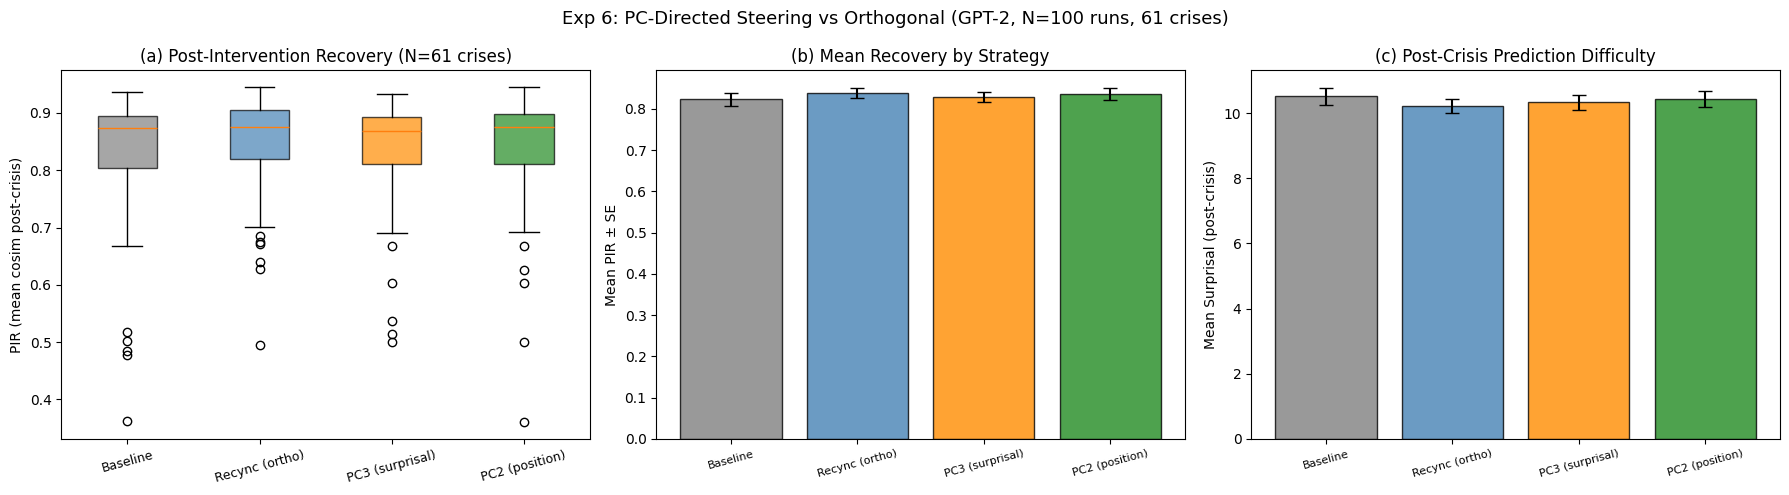
\includegraphics[width=\textwidth]{figures/fig8_steering_n100.png}
\caption{Steering experiment results (GPT-2, $N{=}100$ runs, 61 crisis events). (a)~PIR distributions by strategy---all four conditions are statistically indistinguishable. (b)~Mean PIR with standard error bars---the slight advantage of orthogonal over PC3-directed is not significant. (c)~Post-crisis surprisal is similar across conditions.}
\label{fig:steering}
\end{figure}

This result, now with adequate statistical power ($N = 61$ crisis events), clarifies the role of the geometric decomposition. The PCA axes provide an interpretable coordinate system for \emph{understanding} hidden-state geometry, but targeting specific axes does not improve \emph{intervention} efficacy. If anything, random orthogonal perturbation may be marginally preferable, perhaps because it introduces diversity across multiple representational dimensions simultaneously rather than concentrating the perturbation on a single axis. This is consistent with findings that response-level restart strategies---which induce much larger trajectory changes via seed perturbation---outperform token-level steering \citep{li2024inference}.

\subsection{Why Topology Failed to Discriminate}

The topological analysis yielded a decisive negative result: no non-trivial topology at any PCA dimension or significance threshold. This negative result is informative in two ways.

First, it establishes that the linguistic information encoded in hidden states is \textbf{geometrically but not topologically structured}. The encoding is via linear correlations (positions along principal axes), not via global manifold properties (holes, windings, genus). This is consistent with the success of linear probing methods, which assume that linguistic features are linearly decodable.

Second, it demonstrates a \textbf{methodological caveat} for applying persistent homology to neural network representations: sparsity artifacts dominate when the intrinsic dimensionality is much lower than the ambient PCA dimension. The monotonic increase of $\beta_1$ with PCA dimension, uniform gap ratios near 1.0, and sensitivity of short-text results to threshold selection are all signatures of this phenomenon. We recommend that future applications of persistent homology to neural representations verify robustness to these controls.

% ====================================================================
\section{Limitations}

\begin{enumerate}
    \item \textbf{Model scale.} We validated PC1--norm alignment up to 40B parameters (Falcon-40B, $|r| = 1.000$) across 11 models and five architecture families. Whether this pattern persists in mixture-of-experts architectures or at 70B+ scale remains untested (Llama-2-70B could not be accessed due to gating restrictions). The topology experiments and detailed layer-wise analysis were performed only on models $\leq 7$B.

    \item \textbf{Layer-wise analysis limited to GPT-2.} The layer-wise analysis (Section~4.7) is performed only for GPT-2. Whether the three-phase structure (pre-arc, arc regime, final-layer dissolution) generalizes to other architectures remains to be verified.

    \item \textbf{Simplified POS classification.} Our heuristic POS tagger is coarse (7 categories). Using a proper tagger (e.g., spaCy) would enable finer-grained analysis, potentially revealing structure in currently non-significant components (PC4, PC9).

    \item \textbf{Pre-LN only.} The probing analysis focuses on Pre-LN architectures where PCA concentration is high. The geometric structure of Post-LN hidden states, which do not concentrate on a low-dimensional subspace, remains uncharacterized.

    \item \textbf{Steering experiment.} The intervention experiment (Section~5.4, Table~\ref{tab:steering}) uses only GPT-2. While the sample size ($N = 61$ crisis events from 100 runs) provides adequate power to detect medium effects, generalization to other models and intervention frameworks remains untested.
\end{enumerate}

% ====================================================================
\section{Conclusion}

We investigated the geometry of Pre-LN Transformer hidden-state subspaces using PCA-based probing and persistent homology, across 11 Pre-LN models spanning 124M--40B parameters and five architecture families.

Our experiments suggest that the dominant PCA axis captures hidden-state norm variation, and that removing this axis reveals positional and lexical structure in the residual subspace. In GPT-2, layer-wise analysis shows this structure appearing after the first transformer block and weakening in the final layer. Cross-model comparison across 11 Pre-LN architectures up to 40B parameters shows that PC1--norm alignment holds consistently ($|r| = 1.000$ at 40B scale in Falcon-40B), while positional and POS/difficulty encoding appear consistently but at model-dependent PC indices. Persistent homology finds no evidence of non-trivial topology at the tested scales.

These observations point toward a functional hierarchy---norm, position, lexical difficulty---that may organize Pre-LN hidden-state variation. A preliminary steering experiment found that direction-specific intervention along these axes does not outperform random orthogonal perturbation, suggesting that while the hierarchy is useful for \emph{understanding} representation geometry, exploiting it for \emph{intervention} may require fundamentally different approaches (e.g., response-level restart rather than token-level steering). The apparent topological triviality is consistent with the broad success of linear probing methods, suggesting that Transformer representations encode linguistic structure via linear geometry rather than global topology---though this conclusion is necessarily limited by the model scales and input diversity tested here.

% ====================================================================
\begin{thebibliography}{20}

\bibitem[Aghajanyan et~al.(2021)]{aghajanyan2021intrinsic}
Aghajanyan, A., Gupta, S., and Zettlemoyer, L.
\newblock Intrinsic dimensionality explains the effectiveness of language model fine-tuning.
\newblock In \emph{Proceedings of ACL}, 2021.

\bibitem[Alain and Bengio(2017)]{alain2017understanding}
Alain, G. and Bengio, Y.
\newblock Understanding intermediate layers using linear classifier probes.
\newblock In \emph{ICLR Workshop}, 2017.

\bibitem[Edelsbrunner and Harer(2010)]{edelsbrunner2010computational}
Edelsbrunner, H. and Harer, J.
\newblock \emph{Computational Topology: An Introduction}.
\newblock AMS, 2010.

\bibitem[Ethayarajh(2019)]{ethayarajh2019contextual}
Ethayarajh, K.
\newblock How contextual are contextualized word representations? {C}omparing the geometry of {BERT}, {ELMo}, and {GPT-2}.
\newblock In \emph{Proceedings of EMNLP}, 2019.

\bibitem[Hewitt and Manning(2019)]{hewitt2019structural}
Hewitt, J. and Manning, C.~D.
\newblock A structural probe for finding syntax in word representations.
\newblock In \emph{Proceedings of NAACL}, 2019.

\bibitem[Li et~al.(2018)]{li2018measuring}
Li, C., Farkhoor, H., Liu, R., and Yosinski, J.
\newblock Measuring the intrinsic dimension of objective landscapes.
\newblock In \emph{Proceedings of ICLR}, 2018.

\bibitem[Li et~al.(2024)]{li2024inference}
Li, K., Patel, O., Vi\'{e}gas, F., Pfister, H., and Wattenberg, M.
\newblock Inference-time intervention: Eliciting truthful answers from a language model.
\newblock In \emph{Advances in NeurIPS}, 2024.

\bibitem[Marks and Tegmark(2024)]{marks2024geometry}
Marks, S. and Tegmark, M.
\newblock The geometry of truth: Emergent linear structure in large language model representations.
\newblock \emph{arXiv:2310.06824}, 2024.

\bibitem[Naitzat et~al.(2020)]{naitzat2020topology}
Naitzat, G., Zhitnikov, A., and Lim, L.-H.
\newblock Topology of deep neural networks.
\newblock \emph{Journal of Machine Learning Research}, 21(184):1--40, 2020.

\bibitem[Park et~al.(2024)]{park2024linear}
Park, K., Choe, Y.~J., and Veitch, V.
\newblock The linear representation hypothesis and the geometry of large language models.
\newblock In \emph{Proceedings of ICML}, 2024.

\bibitem[Rieck et~al.(2019)]{rieck2019neural}
Rieck, B., Togninalli, M., Bock, C., Moor, M., Horn, M., Gumbsch, T., and Borgwardt, K.
\newblock Neural persistence: A complexity measure for deep neural networks using algebraic topology.
\newblock In \emph{Proceedings of ICLR}, 2019.

\bibitem[Tenney et~al.(2019)]{tenney2019bert}
Tenney, I., Das, D., and Pavlick, E.
\newblock {BERT} rediscovers the classical {NLP} pipeline.
\newblock In \emph{Proceedings of ACL}, 2019.

\bibitem[Tralie et~al.(2018)]{tralie2018ripser}
Tralie, C., Saul, N., and Bar-On, R.
\newblock Ripser.py: A lean persistent homology library for {P}ython.
\newblock \emph{Journal of Open Source Software}, 3(29):925, 2018.

\bibitem[Turner et~al.(2024)]{turner2024activation}
Turner, A., Thiergart, L., Udell, D., Leech, G., Mini, U., and MacDiarmid, M.
\newblock Activation addition: Steering language models without optimization.
\newblock \emph{arXiv:2308.10248}, 2024.

\bibitem[Xiong et~al.(2020)]{xiong2020layer}
Xiong, R., Yang, Y., He, D., Zheng, K., Zheng, S., Xing, C., Zhang, H., Lan, Y., Wang, L., and Liu, T.
\newblock On layer normalization in the {T}ransformer architecture.
\newblock In \emph{Proceedings of ICML}, 2020.

\bibitem[Zou et~al.(2023)]{zou2023representation}
Zou, A., Phan, L., Chen, S., Campbell, J., Guo, P., Ren, R., Pan, A., Yin, X., Mazeika, M., Dombrowski, A.-K., Goel, S., Li, N., Byun, Z., Wang, Z., Mallen, A., Basart, S., Koyejo, S., Song, D., Fredrikson, M., Kolter, J.~Z., and Hendrycks, D.
\newblock Representation engineering: A top-down approach to {AI} transparency.
\newblock \emph{arXiv:2310.01405}, 2023.

% ── Model references ──

\bibitem[Radford et~al.(2018)]{radford2018improving}
Radford, A., Narasimhan, K., Salimans, T., and Sutskever, I.
\newblock Improving language understanding by generative pre-training.
\newblock \emph{OpenAI Technical Report}, 2018.

\bibitem[Radford et~al.(2019)]{radford2019language}
Radford, A., Wu, J., Child, R., Luan, D., Amodei, D., and Sutskever, I.
\newblock Language models are unsupervised multitask learners.
\newblock \emph{OpenAI Technical Report}, 2019.

\bibitem[Zhang et~al.(2022)]{zhang2022opt}
Zhang, S., Roller, S., Goyal, N., Artetxe, M., Chen, M., Chen, S., Dewan, C., Diab, M., Li, X., Lin, X.~V., Mihaylov, T., Ott, M., Shleifer, S., Shuster, K., Simig, D., Koura, P.~S., Sridhar, A., Wang, T., and Zettlemoyer, L.
\newblock {OPT}: Open pre-trained Transformer language models.
\newblock \emph{arXiv:2205.01068}, 2022.

\bibitem[Biderman et~al.(2023)]{biderman2023pythia}
Biderman, S., Schoelkopf, H., Anthony, Q., Bradley, H., O'Brien, K., Hallahan, E., Khan, M.~A., Purohit, S., Prashanth, U.~S., Raff, E., Skowron, A., Sutawika, L., and van~der~Wal, O.
\newblock {Pythia}: A suite for analyzing large language models across training and scaling.
\newblock In \emph{Proceedings of ICML}, 2023.

\bibitem[Jiang et~al.(2023)]{jiang2023mistral}
Jiang, A.~Q., Sablayrolles, A., Mensch, A., Bamford, C., Chaplot, D.~S., de~las~Casas, D., Bressand, F., Lengyel, G., Lample, G., Saulnier, L., Lavaud, L.~R., Lachaux, M.-A., Stock, P., Le~Scao, T., Lavril, T., Wang, T., Lacroix, T., and El~Sayed, W.
\newblock {Mistral} 7{B}.
\newblock \emph{arXiv:2310.06825}, 2023.

\bibitem[Yang et~al.(2024)]{yang2024qwen2}
Yang, A., Yang, B., Hui, B., Zheng, B., Yu, B., Zhou, C., Li, C., Li, C., Liu, D., Huang, F., et~al.
\newblock {Qwen2} technical report.
\newblock \emph{arXiv:2407.10671}, 2024.

\bibitem[Almazrouei et~al.(2023)]{almazrouei2023falcon}
Almazrouei, E., Alobeidli, H., Alshamsi, A., Cappelli, A., Cojocaru, R., Debbah, M., Goffinet, \'{E}., Hesslow, D., Launay, J., Malartic, Q., Mazzotta, D., Penedo, G., and Muennighoff, N.
\newblock The {Falcon} series of open language models.
\newblock \emph{arXiv:2311.16867}, 2023.

\end{thebibliography}

% ====================================================================
\appendix
\section{Experimental Details}

\subsection{Software and Hardware}

All experiments were run on Apple M1 (16\,GB RAM) using Python~3.13, PyTorch~2.11, Transformers~5.4, scikit-learn~1.8, ripser~0.6, and scipy~1.17. Total computation time for all experiments was under 10 minutes. The cross-model comparison (Section~5.1) additionally requires downloading Pythia-410M, Qwen2-0.5B, and OPT-1.3B from HuggingFace Hub.

\subsection{Reproduction}

\begin{verbatim}
cd manifold_topology_experiment
python -m venv .venv && source .venv/bin/activate
pip install -r requirements.txt

# Topology (Section 4.1)
python experiments/topology/exp2_persistent_homology.py
python experiments/topology/exp2b_topology_deep_dive.py
python experiments/topology/exp2c_highd_long_text.py

# Probing (Sections 4.2-4.7)
python experiments/probing/exp5_thickness_probing.py
python experiments/probing/exp5b_norm_normalized.py
python experiments/probing/exp5c_layerwise.py
python experiments/probing/exp5d_cross_model.py
\end{verbatim}

The 7B+ experiments (Sections~5.1, 5.3) and the steering experiment (Section~5.4) require GPU and were conducted on Google Colab; scripts are in \texttt{colab/}.

\subsection{PCA Calibration Stability}

PCA components were computed per-text, per-model. The cross-text replicability of PC--feature associations (Table~\ref{tab:probing}) confirms that the principal directions are stable properties of the model architecture rather than artifacts of specific input texts.

\end{document}
